\documentclass[]{report}   % list options between brackets


% Latex Police and file encoding
\usepackage[utf8]{inputenc}
\usepackage[T1]{fontenc}  % for character encoding 
\usepackage{lmodern}  % Police setting
\usepackage[frenchb]{babel}
% Graphics inclusion
\usepackage{graphicx}

% Code Formating
% For code snippets style definition

\usepackage{color}
\usepackage{listings}


\lstloadlanguages{[ISO]C++,C,bash}
% set up listing environment with C syntax hightlight
\definecolor{stringcolor}{rgb}{0.20,0.50,0.20}
\definecolor{commentcolor}{rgb}{0.40,0.40,0.40}
\definecolor{keywordcolor}{rgb}{0.50,0.10,0.10}
\definecolor{idcolor}{rgb}{0.10,0.10,0.50}
\definecolor{bg}{rgb}{0.95,0.95,0.95}
% with \lstset one can predefine parameters for listings
\lstset{language=[ISO]C++,basicstyle=\small,keywordstyle=\color{keywordcolor},
        commentstyle={\color{commentcolor}\itshape},
        stringstyle={\color{stringcolor}},
        identifierstyle=\color{idcolor},numbers=left,
       % xleftmargin=2em,framerule=0.8pt,
        stepnumber=1,
        frame=single,
        showstringspaces=false,
        firstnumber=1,
        numberstyle=\ttfamily,backgroundcolor=\color{bg},
        basicstyle=\ttfamily\footnotesize}
        
        
% Definition of \C++ to be eye candy :
\usepackage{relsize}
\usepackage{lipsum}
%c from texinfo.tex
\def\ifmonospace{\ifdim\fontdimen3\font=0pt }
\def\C++{%
\ifmonospace%
    C++%
\else%
    C\kern-.1667em\raise.30ex\hbox{\smaller{++}}%
\fi%
\spacefactor1000 }

%Inliine listings :
\usepackage{paralist}

%figures :
\usepackage{graphicx}
\usepackage{float}
\floatstyle{boxed} %border around figures
\restylefloat{figure}
\usepackage[format=plain,indention=.5cm,parskip=5pt,bf]{caption}
%import section
\usepackage{wrapfig}


%TODO macro
\newcommand{\TODO}[1] {\marginpar{\colorbox{red}{\Huge \textbf{TODO}} } \colorbox{red}{\Huge \textbf{TODO}}\colorbox{green}{\normalsize #1  } } 

% Hypertext links
\usepackage[colorlinks=true,breaklinks=false,dvips,ps2pdf]{hyperref}
\urlstyle{sf}




\begin{document}

\title{Projet de Fin d'Étude} 
\author{Antonin PERROT-AUDET
  Institut National des Sciences Appliquées,\\
  Lyon,\\
  France,\\
  \texttt{antonin.perrot-audet@insa-lyon.fr}}   
\date{Février-Septembre, 2010} 
\maketitle


\begin{abstract}
  Ce rapport présente le travail effectué pendant mon Projet de Fin d'Étude (PFE) au sein du Megason Lab, Harvard Medical School, Boston MA, USA. Ce PFE conclut ma formation à l'Institut National des Sciences Appliquées de Lyon, au département Génie Électrique, pour acquérir le grade d'Ingénieur INSA. Il s'agit aussi d'un stage de recherche finalisant le master Génie Électrique et des Procédés, parcours Systèmes et Images à l'INSA de Lyon, l'École Centrale de Lyon, et l'Université Claude Bernard Lyon 1.

  Le travail a pour thème le traitement d'images microscopiques. Il s'agit de vidéos tri-dimensionnelles du poisson zèbre durant sa phase de développement embryonnaire. Le laboratoire inclut une équipe d'informaticiens développant un programme à l'usage des biologistes : {\gofigure}\cite{refGofigure2}. A terme, les résultats théoriques devront être intégrés à ce logiciel .
  
  
\tableofcontents  
  
 
\end{abstract}


\chapter{Description du Megason lab et de ses objectifs} 
\phantomsection
\addcontentsline{toc}{chapter}{Description du Megason lab et de ses objectifs} 

\section{Le Megason Lab}

\subsection{L'équipe du laboratoire}
Le Megason lab est un laboratoire dont le personnel est composé de chercheurs post-doctorants.
Il y a clairement deux domaines d'expertise : Biologie, et Informatique.
L'équipe de biologistes mène des recherches sur le développement du poisson zèbre,
tandis que l'équipe d'informaticiens développe un programme de visualisation,
segmentation, suivi de cellules adapté aux données de la microscopie.

{\small \begin{tabular*}{1.0\textwidth}{@{\extracolsep{\fill}} |  p{2.5cm} |  p{3.cm} | p{3.5cm} | c | }
\hline Nom & Poste & Intérêts & Nationalité \\ 
\hline Sean Megason & Professeur (Docteur) & Financement et management du laboratoire. & USA \\ 
\hline Ramil Noche & Séjour Postdoctoral & Formation du système nerveux. & Philipines \\ 
\hline Fengzhu Xiong & Étudiant en thèse & Création d'un poisson ayant une couleur différente par cellule. & Chine \\ 
\hline Nikolaus Obholzer & Séjour Postdoctoral & Développement de l'oreille et création de marqueurs génétiques fluorescents. &  Allemange \\ 
\hline Paul Cowgill & Étudiant en thèse & Effet des drogues sur le poisson zèbre. & USA \\ 
\hline David Tulga & Étudiant en thèse & Développement cellulaire. &  USA \\ 
\hline Ian Swiburne & Séjour Postdoctoral & Développement de l'oreille du poisson zèbre. & USA \\ 
\hline Andrea Tentner & Séjour Postdoctoral & Différenciation des cellules provenant d'un ancêtre commun. & USA \\ 
\hline Amelia Green & Séjour Postdoctoral & Formation des oreilles du poisson zèbre. & Angleterre \\ 
\hline Evan Schwab & Associe & Séquences du code génétique du poisson zèbre. & USA \\ 
\hline Dante D'India & Technicien & Entretient des animaux. & USA \\ 
\hline Arnaud Gelas & Ingénieur de recherche (senior) & Programmation de {\gofigure} : Management du projet. &  France \\
\hline Kishore Mosaliganti & Séjour Postdoctoral & Algorithmes de traitement de l'image, recalage et segmentation. & Inde \\ 
\hline Lydie Souhait & Ingénieur de recherche & Programmation de {\gofigure} : Responsable de la base de donnees (design, connexion, requetes), et GUI & France \\
\hline Nicolas Rannou & Ingénieur de recherche & Programmation de {\gofigure} : Responsable de la visualisation dans {\gofigure} & France \\
\hline Antonin Perrrot-Audet & Stagiaire en PFE & Traitement d'image : Segmentation des cellules; Programmation de {\gofigure} & France \\
\hline 
\end{tabular*} }

Il est important de noter que le Megason lab bénéficie des infrastructures et services du département Systems Biology de Harvard Medical School.


\subsection{Les objectifs du laboratoire}
L'objectif principal du Megason lab, est de comprendre les premières étapes du développement animal.
L'idée étant d'assimiler le génome à un programme informatique.
En modifiant le code génétique d'organismes vivants, et en observant le développement cellulaire,
les biologistes parviennent à identifier les acteurs intervenant dans le développement de l'embryon, et à comprendre leur fonction.

Les expériences sont réalisées sur des poissons zèbres.
De la même manière qu'un informaticien introduit des "breakpoints" dans un programme pour intervenir dans son exécution,
les biologistes créent des poissons mutants et analysent les effets des modifications du génome sur le développement.
L'étape suivante consistera à créer un modèle du développement du poisson zèbre.
En ce moment, les centres d'intérêts de l'équipe de biologiste sont la formation du système nerveux, et des oreilles.

Les biologistes recueillent d'énormes quantités de données
correspondant à des vidéos d'embryons de poissons zèbres (typiquement, 150Giga bytes par vidéo).
Afin de pouvoir exploiter ces données,
une équipe de développeurs informatiques a été formée.
Cette équipe a pour objectif de développer la prochaine plateforme
pour l'analyse d'images de microscopie: {\gofigure}.
Il s'agit donc de créer une application extrêmement accessible ("cross-platform
\footnote{Un logiciel multiplate-forme ou multiplateforme est un logiciel conçu pour fonctionner sur plusieurs plates-formes, c'est-à-dire le couple liant ordinateur et système d'exploitation. En anglais on parle souvent de "cross-platform software" ou "platform independent software" ou encore de "multi-platform software".}
"), 
avec un code de qualité,
et distribué gratuitement ("open-source
\footnote{La désignation open source (au Québec : "code source libre") s'applique aux logiciels dont la licence respecte des critères précisément établis par l'Open Source Initiative, c'est-à-dire la possibilité de libre redistribution, d'accès au code source et de travaux dérivés.}
"),
pour permettre l'implication aisée de nouveaux chercheurs
en traitements de l'images et d'informaticiens.

\subsection{Le Matériel} 
Le Megason lab dispose d'équipements récents et perfectionnés, tant dans le domaine de la biologie que de l'informatique. Le personnel d'Harvard assure sa prise en charge et son entretien.
Pour mon PFE, je me suis plutôt intéressé aux dispositifs d'acquisition et de traitement d'image : les microscopes et les ordinateurs.

\subsubsection{Les dispositifs d'imagerie}


Le Megason lab dipose de nombreux microscopes pour permettre aux biologistes de mener à bien leurs manipulations sur les poissons zèbres.
L'équipe de traitement de l'image s'intéresse plutôt aux images produites par le microscope confocal deux-photons à plateau automatisé. 

Les techniques d'imagerie au Megason Lab sont basées sur des marqueurs fluorescents fixés sur certaines molécules du spécimen (l'embryon de poisson zèbre à différentes étapes de son développement). Les atomes de ces phosphores doivent être excités afin d'émettre de la lumière.


Le principe du microscope confocal (illustré par la figure~\ref{fig:ConfocalPrinciple}) est d'illuminer (exciter) seulement le point que l'on observe : la lentille d'illumination est aussi la lentille d'observation, on illumine donc le plan focal de cette lentille. Cela permet de concentrer l'énergie lumineuse sur le plan observé (plan focal). De plus, afin de limiter l'impact des plans non observés, un diaphragme est ajouté à l'objectif d'observation.

Le microscope confocal dont nous disposons est un microscope deux-photons (figure~\ref{fig:Confocal2photonsPrinciple}).
Cela s'signifie que l'illumination du point observé est faite par deux rayons lumineux convergents.
Cette technique a plusieurs avantages :
\begin{itemize}
  \item Le phosphore a besoin de l'énergie de deux photons pour émettre de la lumière. En dehors du point focal, il n'y a jamais assez d'énergie apportée : seuls les atomes des phosphores focalisés peuvent émettre de la lumière. On accroit ainsi énormément la résolution.
  \item La longueur d'onde d'excitation est approximativement deux fois plus grande que celle d'un microscope confocal traditionnel, et pénètrent donc mieux les tissus : on peut analyser des spécimens épais.
  \item Chacun de ces deux rayons transporte moins d'énergie que si il y avait eu un seul rayon pour illuminer le point observé.
  Ainsi, il y a moins de dommages causés au spécimen observé.
\end{itemize}

Il est pour l'instant possible d'utiliser trois marqueurs fluorescents différents à la fois, que l'on stocke dans une image multicolore.
Ce microscope a été assemblé au Megason Lab à partir d'un microscope Zeiss 710 NLO (figure~\ref{fig:MicMegason}).
Une chambre environnementale a été créée, afin de contrôler le développement des embryons durant la capture d'informations.

\begin{figure}[htb]
\begin{center}
\leavevmode
\includegraphics[width=0.95\textwidth]{pictures/ConfocalPrinciple}
\end{center}
\caption{Principe du microscope confocal (source :\href{http://en.wikipedia.org/wiki/File:Confocalprinciple.svg}{Wikipedia})}
\label{fig:ConfocalPrinciple}
\end{figure}

\begin{figure}[htb]
\begin{center}
\leavevmode
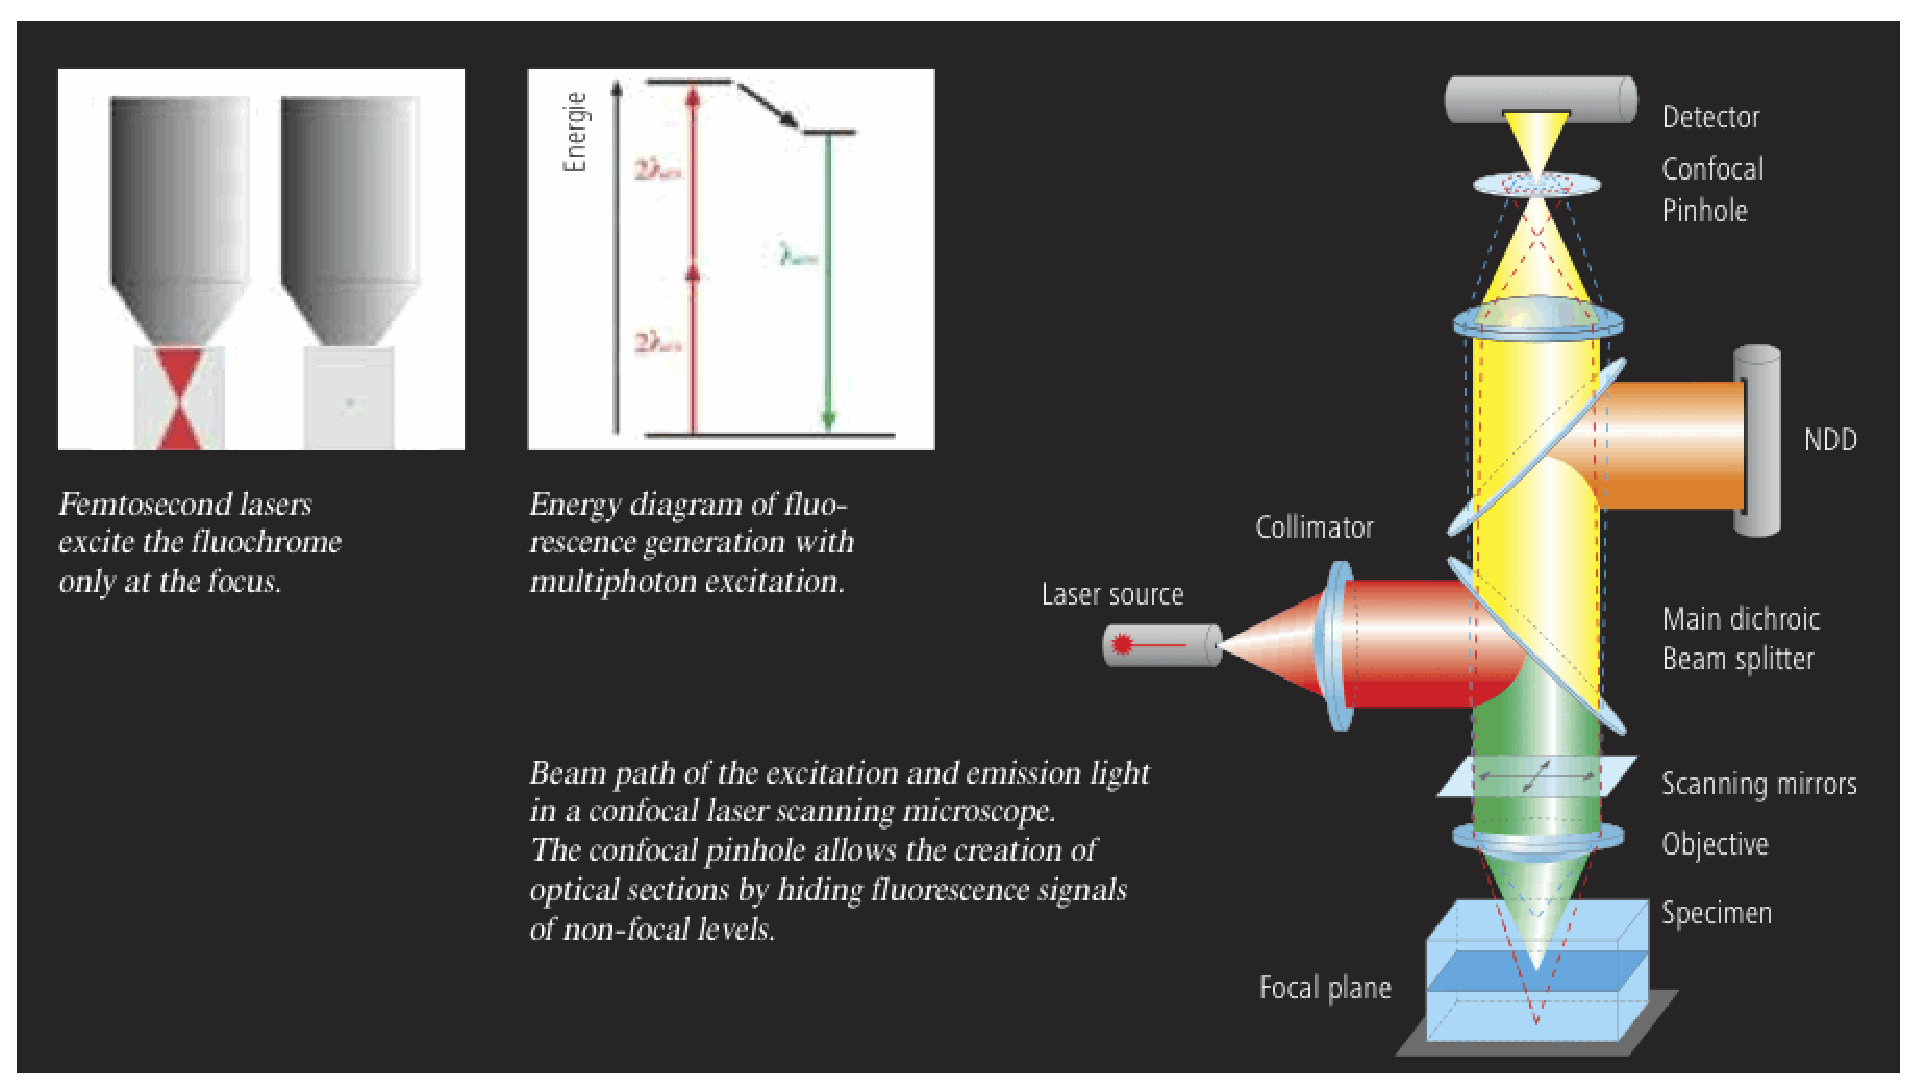
\includegraphics[width=0.95\textwidth]{pictures/ConfocalZeissPrinciple}
\end{center}
\caption{Principe du microscope confocal 2 photons utilisé (Zeiss documentation)}
\label{fig:Confocal2photonsPrinciple}
\end{figure}

\begin{figure}[htb]
\begin{center}
\leavevmode
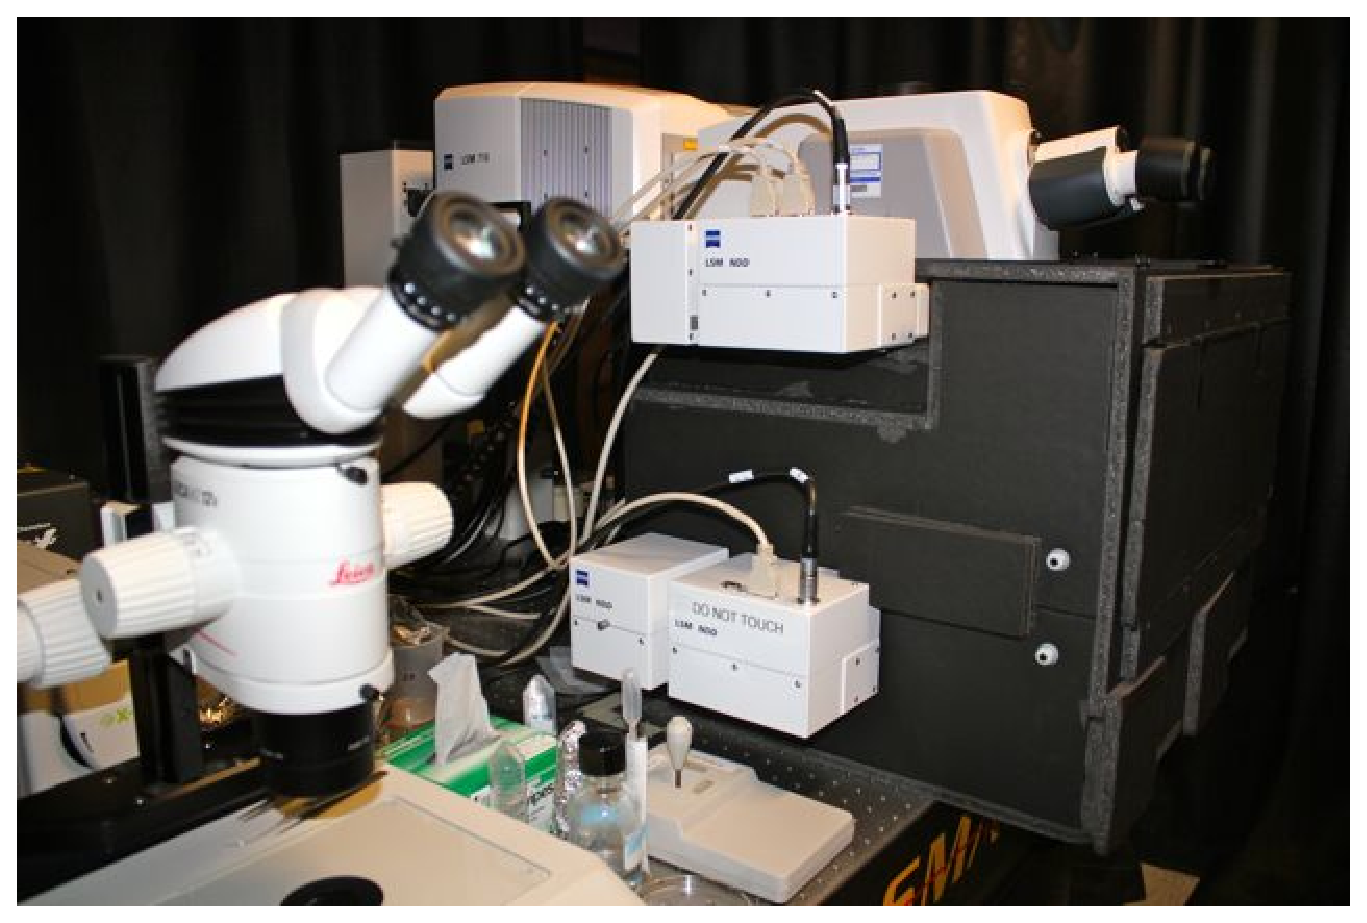
\includegraphics[width=0.95\textwidth]{pictures/PICmicroscope}
\end{center}
\caption{Microscope confocal 2-photons Zeiss 710 NLO utilisé au Megason Lab}
\label{fig:MicMegason}
\end{figure}

\clearpage


% Chapitre sur le rapport d ingenierie :

\chapter{Rapport d'ingénierie}


\section*{Introduction}
Ce PFE conclut les cinq années d'étude à l'INSA de Lyon. 
Il s'agit de démontrer des capacités d'adaptation,
d'innovation et d'initiative propres à un ingénieur.

Les laboratoires ont besoin de l'expertise d'ingénieurs
pour résoudre des problème techniques, qui se posent du fait de l'utilisation de matériel hautement sophistiqué.
Notamment, au Megason Lab, ce sont principalement des ingénieurs qui développent le programme de visualisation de données. 
Les problèmes d'acquisitions d'images biologiques révèlent aussi des défis techniques.
 
\section*{Objectifs}

Les objectifs initiaux étaient centrés principalement sur la recherche.
Cependant, le Megason lab cherche au maximum à intégrer les avancées en traitement de l'image aux outils qu'il conçoit,
 notamment au programme \gofigure. Cela entraine des contraintes vis à vis des outils de développements. 
 Il a donc fallu me former afin que je devienne un programmeur avancé en {\C++}. 
 
J'ai ainsi commencé mon PFE en tant que membre de l'équipe de développement de {\gofigure}.
 Les objectifs étant d'utiliser les différentes librairies dont se sert le programme, pour mettre au point un système de plugins
 \footnote{En informatique, un plugin ou plug-in (aussi nommé module d'extension, greffon ou plugiciel au Québec) est un logiciel qui complète un logiciel hôte pour lui apporter de nouvelles fonctionnalités. Notamment, pour le logiciel \gofigure, les plugins seront des algorithmes de traitement d'images.}. 
 Ma mission était de créer une librairie de comparaison d'images, afin d'inclure aux plugins, un aperçu, de la même manière que Gimp\footnote{Gimp vient de GNU Image Manipulation Program (GIMP). Gimp est un programme de retouche d'images gratuit et open-sources.
 }, qui affiche un aperçu pour ses filtres.

Dans le cadre de ma participation au développement de \gofigure,
 j'ai aussi proposé un protocole de travail avec un nouveau programme de gestion de versions : Git.
 Il s'agissait tout d'abord d'apprendre à utiliser Git, pour ensuite transmettre ce savoir et enfin proposer une méthode de travail.

Mon PFE étant motivé par des objectifs de traitement de l'image, j'ai aussi travaillé sur l'amélioration
 des techniques d'acquisitions de données microscopiques.
 
 
\section*{Planning} 
 
Des objectifs, nous pouvons dégager des tâches, que nous plaçons dans un diagramme de Gantt. Le diagramme présenté figure~\ref{fig:GanttPFEInge}, ne concerne que les tâches d'ingénierie, or le PFE était aussi un stage master avec des objectifs recherche. Le diagramme de Gantt général du PFE est donc présenté en annexe~\ref{AnnexeGanttGlobal}.
 
\begin{figure}[h]
\begin{center}
\leavevmode
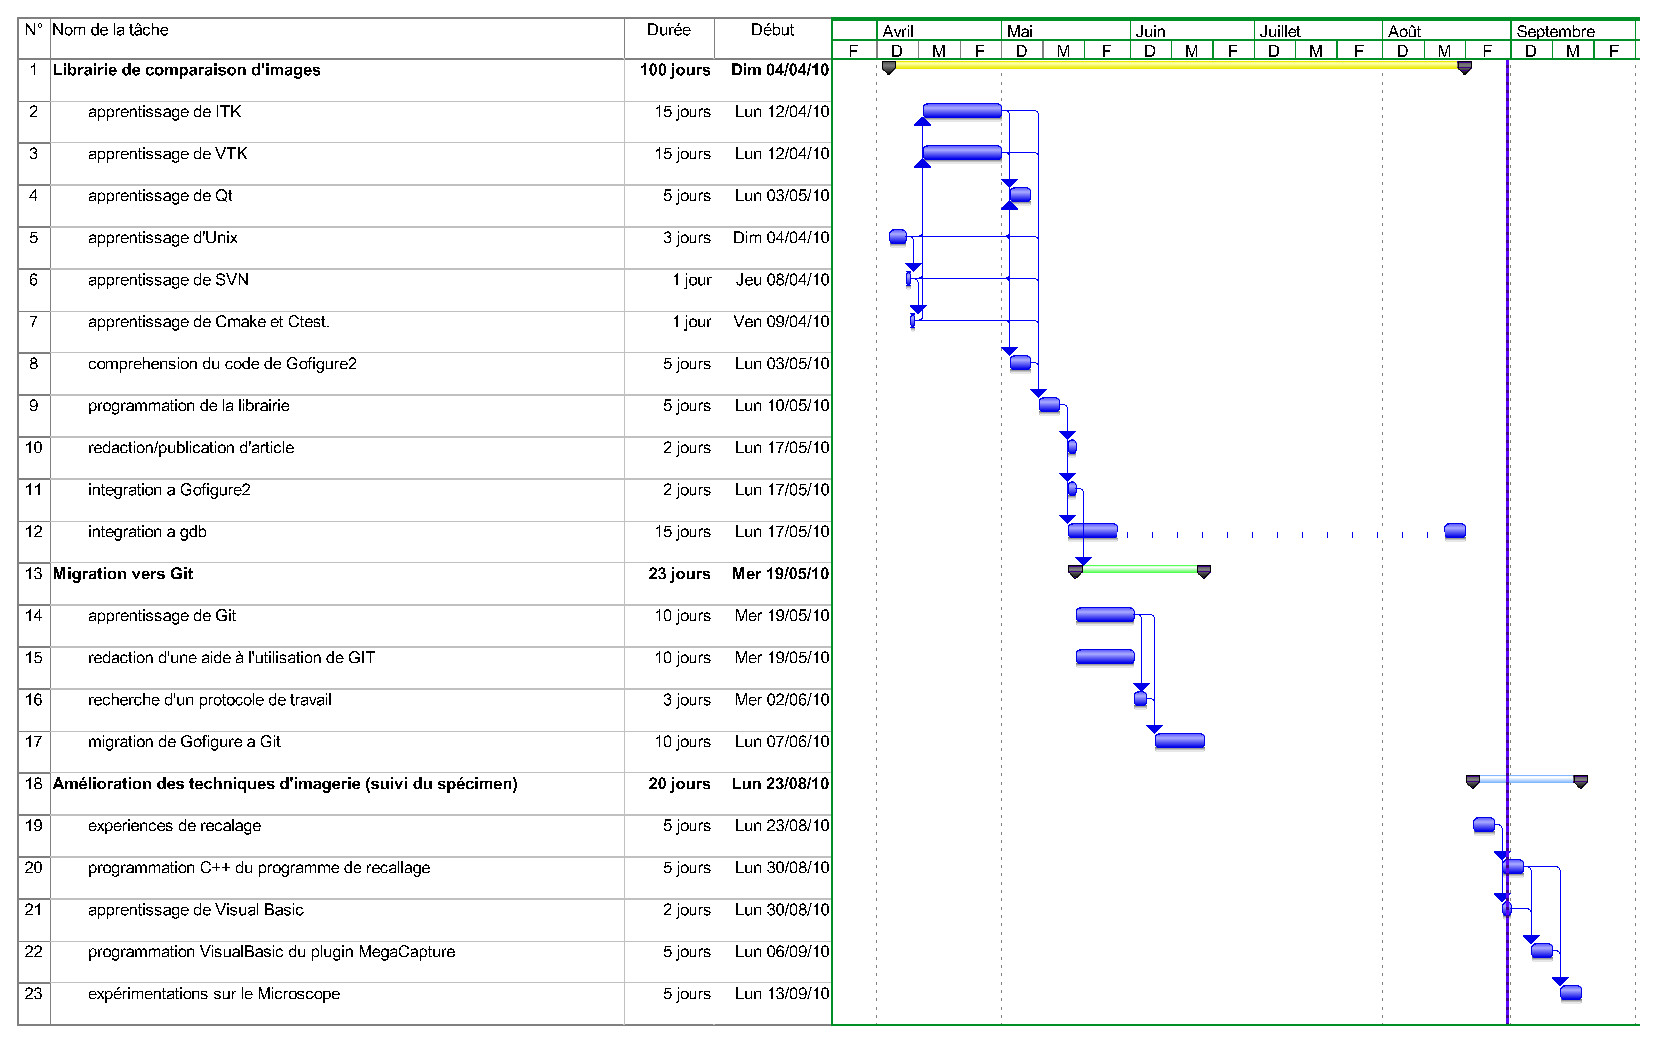
\includegraphics[angle=-90, width=0.95\textwidth]{pictures/GanttPFEInge}
\end{center}
\caption{Gantt de la partie ingénierie du PFE}
\label{fig:GanttPFEInge}
\end{figure}

%--------------------------------------------------
%             COMPARAISON
%--------------------------------------------------


\section{Création d'une librairie \\ de comparaison d'images}

L'équipe d'informaticiens au Megason Lab est divisée en deux : deux ingénieurs travaillent sous la direction d'un docteur sur la
 création de l'outil de visualisation d'images microscopiques (\gofigure), tandis qu'un autre docteur travaille sur
 des algorithmes de traitement d'image. Afin de travailler pour l'ensemble des informaticiens, le projet a deux objectifs
\begin{inparaenum}[(i)]
  \item faciliter le travail de développement d'algorithmes de traitement de l'image, et 
  \item s'intégrer au développement de {\gofigure}.
\end{inparaenum}

La création de la librairie de comparaison d'images atteint ces deux buts (i) et (ii):\\ 
Il s'agit d'un programme utilisant le code source du projet {\gofigure}, 
qui sera utilisé pour le développement des plugins de {\gofigure}.
Une autre application de cette librairie complète le projet de débugueur graphique de 
Matthiew MacCormick \cite{McCornic-VisualDebug}. Nous rendons ainsi cette librairie particulièrement utile
aux développeurs.
Ce programme permet aussi de visualiser les traitements appliqués aux données
lors de l'exécution d'un algorithme de traitement d'images sous un environnement de debugging (gdb
\footnote{Un débogueur, débugueur ou encore debugger (de l'anglais), est un logiciel qui aide un développeur à analyser les bugs d'un programme. Pour cela, il permet d'exécuter le programme pas-à-pas, d'afficher la valeur des variables à tout moment, de mettre en place des points d'arrêt sur des conditions ou sur des lignes du programme ...\\
Le GNU Debugger également appelé gdb est le débogueur standard du \href{http://fr.wikipedia.org/wiki/Projet_GNU}{projet GNU}.} ).


\subsection{Cahier des charges}

Nous spécifions l'ensemble des tâches réalisées au cours du PFE avec la méthode APTE{\textregistered}{\cite{methodeAPTE}}. Celle ci nous permet de définir les fonctions à remplir pour parvenir à un objectif. L'objectif est spécifié par le diagramme Bête à cornes (figure~\ref{fig:BACCompare}), tandis que les fonctions sont décrites dans l'analyse du diagramme pieuvre(figure~\ref{fig:PIEUVRECompare}).

\begin{figure}[h]
\begin{center}
\leavevmode
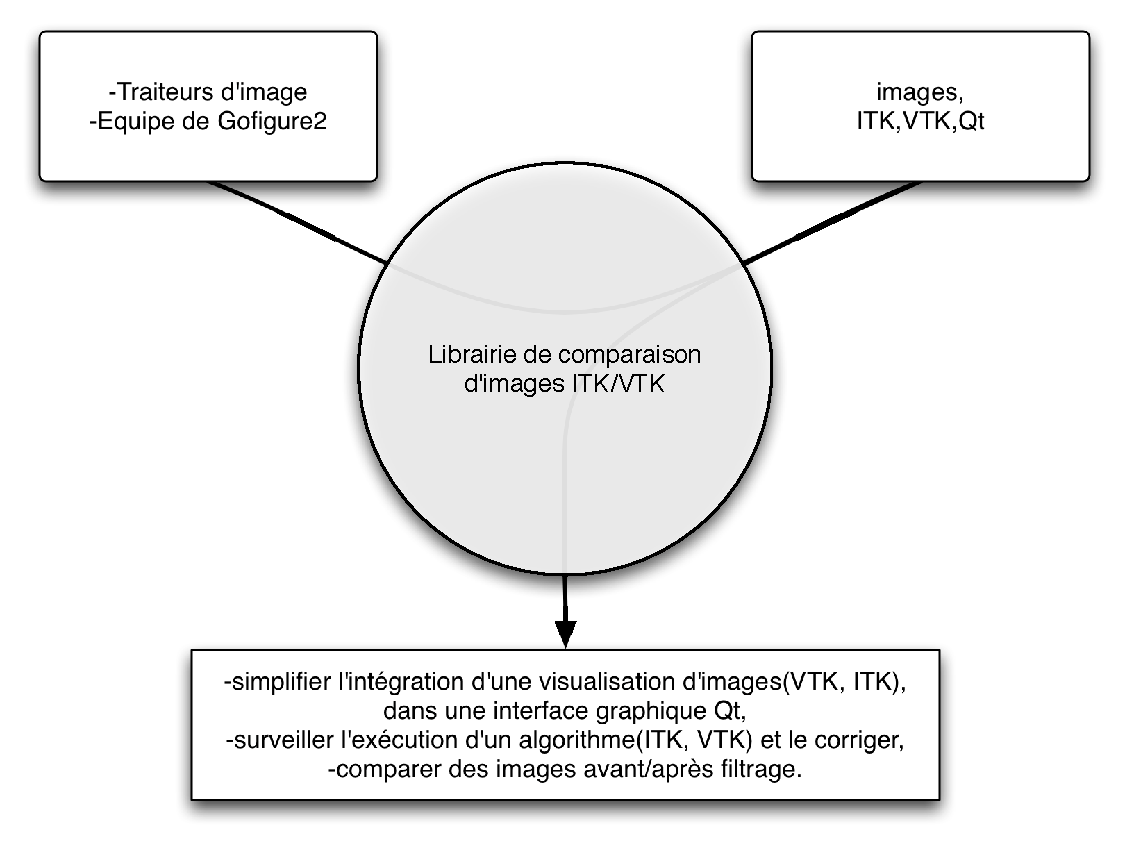
\includegraphics[width=0.95\textwidth]{pictures/CompareBAC}
\end{center}
\caption{Bête à cornes (méthode {APTE\textregistered}) de la librairie de comparaison d'images}
\label{fig:BACCompare}
\end{figure}

L'analyse de la Bête à cornes consiste à répondre aux questions :
\begin{inparaenum}[(i)] 
  \item pourquoi cherche-t'on à atteindre ce but ?
  \item et qu'est ce qui pourrait faire disparaitre ou évoluer le projet ?
\end{inparaenum}

Le programme {\gofigure} va bientôt disposer d'une interface pour créer des plugins afin de traiter des images microscopiques.
Le développement d'une librairie de visualisation et de comparaison est donc nécessaire
pour contrôler les paramètres des algorithmes inclus dans les plugins.

De plus, lors du développement d'algorithmes,
il est souvent nécessaire, lors de la phase de test et d'évaluation,
de visualiser l'état des données traitées, pendant l'exécution du programme.
Les algorithmes sont la plupart du temps prototypés en \C++ au Megason Lab, et la visualisation de données n'est pas triviale.
Il faut souvent ajouter une dizaine de lignes de codes pour pouvoir sauvegarder une image.
Une telle tâche est fastidieuse, et ce projet permettrait de visualiser
des données lors de l'exécution du programme, sans rajouter de code ni de le recompiler !\\

De par mon implication dans l'équipe de {\gofigure} et
comme je vais être amené à développer des algorithmes en {\C++},
coder une librairie de comparaison d'images me permettra de me former aux outils utilisés au Megason Lab,
tout en créant un outil indispensable pour mes travaux futurs.

\begin{figure}[h]
  \begin{center}
  \leavevmode
  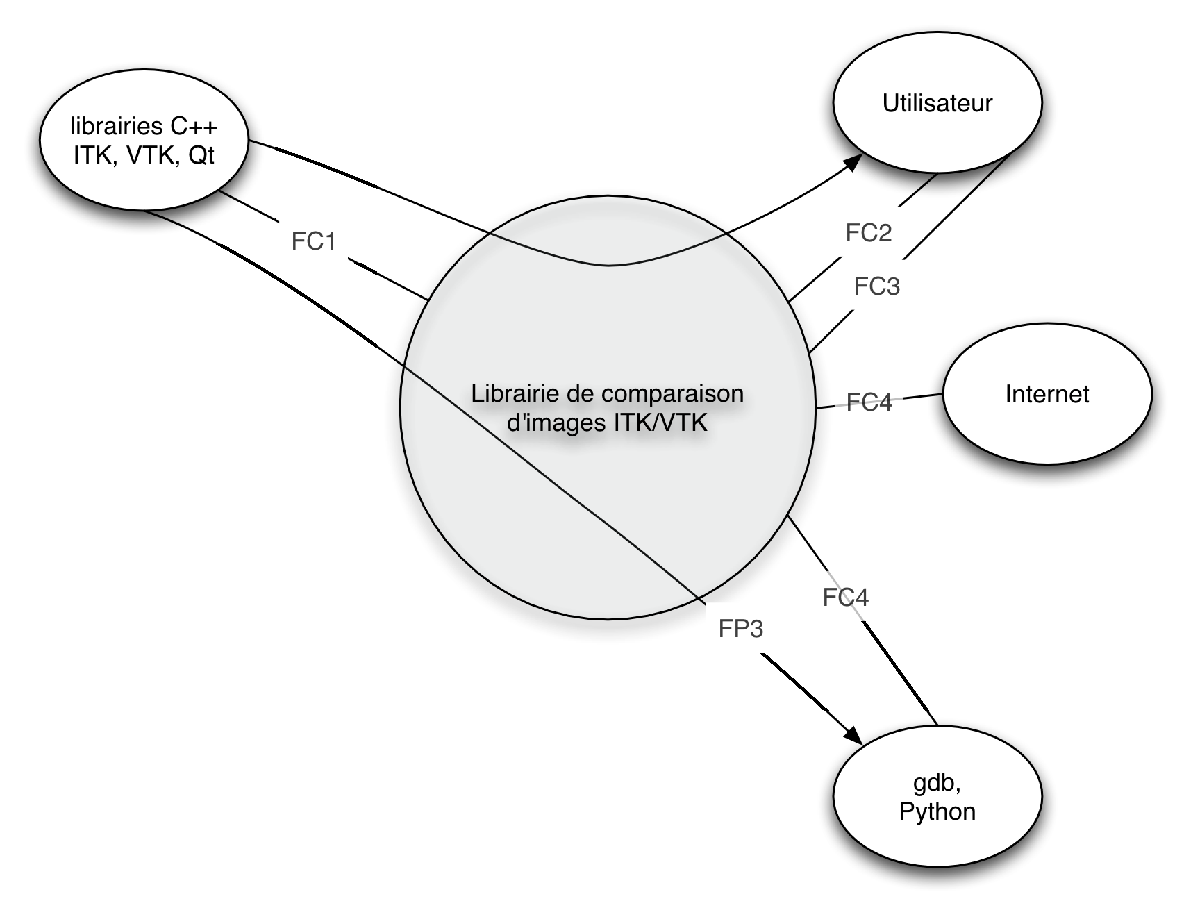
\includegraphics[width=0.95\textwidth]{pictures/ComparePIEUVRE}
  \end{center}
  \caption[Diagramme Pieuvre (méthode {APTE\textregistered}) de
    la librairie de comparaison d'images]{Diagramme
    Pieuvre (méthode {APTE\textregistered})
    de la librairie de comparaison d'images
  \small
  \textbf{Fonctions principales :}\\
  FP1 : visualiser des données (fichiers ou en mémoire) provenant 
    de VTK et ITK dans Qt\\
  FP2 : synchroniser la visualisation de plusieurs images\\
  FP3 : débuguer visuellement des pipelines ITK et VTK dans gdb\\
    \textbf{Fonctions contraintes :} \\
  FC1 : être compatible avec VTK, ITK et Qt\\
  FC2 : proposer une interface simple, une documentation, des exemples, et être
    facilement modifiable\\
  FC3 : être visible sur internet\\
  FC4 : être compatible avec Python pour interfacer avec gdb}
  \label{fig:PIEUVRECompare}
\end{figure}


\clearpage


Une analyse du diagramme pieuvre est ensuite donnée. Nous répondons aux questions de la méthode {APTE\textregistered}, pour chaque fonction :
\begin{inparaenum}[(i)] 
  \item dans quel but existe-t-elle ?
  \item à cause de quoi existe-t-elle ?
  \item pourrait-elle évoluer ou disparaitre ?
\end{inparaenum}


\paragraph*{FP1} :\\ visualiser des données (fichiers ou en mémoire) provenant de VTK et ITK dans Qt
\begin{itemize}
  \item Existe pour afficher les résultats des traitements réalisés par des plugins ITK/VTK dans {\gofigure}.
  \item Existe à cause de la nécessité pour l'utilisateur d'avoir une visualisation dans une interface construite.\\
  Existe du fait de la complexité actuelle de l'utilisation d'ITK et VTK avec Qt. 
  \item Pourrait disparaitre si une librairie plus efficace et simple de visualisation était crée.
\end{itemize}

\paragraph*{FP2} :\\ synchroniser la visualisation de plusieurs images
\begin{itemize}
  \item Existe pour comparer pixel(voxel) par pixel plusieurs images.
  \item Existe à cause du besoin des traiteurs d'image d'une telle comparaison.
  \item Pourrait évoluer si VTK ou le moteur 3D utilisé MegaVTK (développé à partir de vtkINRIA3D\cite{vtkINRIA})
  proposaient des solutions simple de synchronisation de visualisations.
\end{itemize}

\paragraph*{FP3} :\\ débuguer visuellement des pipelines ITK et VTK dans gdb
\begin{itemize}
  \item Existe pour permettre au programmeur de rapidement visualiser des images
   à différents points d'une pipeline ITK ou VTK.
  \item Existe à cause du besoin de débuguer les algorithmes de traitement d'image,
  et de visualiser les images d'une manière compréhensible par un humain.
  \item Pourrait évoluer si ITK, gdb ou Python évoluent.
\end{itemize}

\paragraph*{FC1} :\\ être compatible avec VTK, ITK et Qt
\begin{itemize}
  \item Existe pour permettre à l'application de fonctionner.
  \item Existe car ces 3 librairies sont complémentaires et souvent utilisées conjointement dans une même application.
  \item Pourrait disparaitre si une librairie regroupant les fonctions d'ITK, VTK et Qt était crée, et si {\gofigure} l'utilisait.
\end{itemize}

\paragraph*{FC2} :\\ Proposer une interface simple, une documentation, des exemples, et être facilement modifiable
\begin{itemize}
  \item Existe pour permettre à un utilisateur d'utiliser, comprendre et modifier la librairie.
  \item Existe à cause du fait qu'un code mélant ITK, VTK, et Qt n'est pas trivial.
  \item Pourrait évoluer avec la librairie.
\end{itemize}

\paragraph*{FC3} :\\ être visible sur internet
\begin{itemize}
  \item Existe pour permettre à un maximum de programmeur de télécharger la librairie et l'utiliser.
  \item Existe car la librairie est open-source et s'améliore avec les contributions d'autres utilisateurs.
  \item Pourrait disparaitre si la librairie venait à ne plus être publique.
\end{itemize}

\paragraph*{FC4} :\\ être compatible avec Python pour interfacer avec gdb
\begin{itemize}
  \item Existe pour permettre l'intégration à gdb et le débuguage visuel des pipelines ITK et VTK.
  \item Existe car le débugueur gdb nécessite une interface python 
  pour interpréter les données en provenance 
  des pipelines ITK et VTK dans un programme externe.
  \item Pourrait disparaitre si gdb n'utilisait plus Python 
  pour interfacer avec des programmes externes.
\end{itemize}

\subsection{Les outils utilisés}
Afin de pouvoir programmer ce projet,
il a été nécessaire d'apprendre à utiliser un certain nombre d'outils,
de librairies et concepts {\C++}. Cet apprentissage a été une
partie importante de mon PFE, me permettant d'acquérir de
nouvelles compétences en sciences informatiques.
\subsubsection{Les librairies \C++}
Il existe un grand nombre de fonctions déjà codées en {\C++}.
Dans une optique de standardisation et d'efficacité, il est important d'apprendre
à utiliser des librairies contenant les fonctions utiles au programme que l'on crée.

Le projet utilise trois grandes librairies open-source et cross-platform :
\begin{description}
  \item[Insight ToolKit (ITK)] qui est spécialisée dans le traitement d'image. Nous utilisons cette librairie, 
  afin de supporter le type de données qu'elle stocke en mémoire.
  \item[Visualization ToolKit (VTK)] qui est spécialisée dans la visualisation d'images. 
  Nous utilisons cette librairie afin de supporter le type de données qu'elle stocke en mémoire,
  et aussi pour visualiser les données acquises par la librairie.
  \item[Qt]\cite{refQT} qui est spécialisée dans la création d'interfaces graphiques. 
  Nous avons rendu notre travail directement compatible avec cette librairie
  pour permettre aux utilisateurs de l'intégrer dans n'importe quelle application développée avec Qt.
  \item[vtkINRIA3D]{\cite{vtkINRIA}} qui est le moteur 3D de {\gofigure}\cite{refGofigure2}.
  Cette librairie permet d'explorer un volume tri-dimensionnel en affichant trois coupes selon des plans perpendiculaires.
  Simultanément, un objet tridimensionnel composé par ces trois coupes est affiché.
  La version présente dans {\gofigure} à été grandement modifiée et renommée MegaVTK.
\end{description}
Une description détaillée de ces librairies est présentée en annexe~\ref{AnnexeDescriptionITKVTKQT}.


\subsubsection{Les outils de programmation}
A partir d'un certain niveau, en {\C++}, il est indispensable de maitriser certains outils complexes. Ceux-la, après un temps
 d'apprentissage, augmentent grandement la productivité.
Les outils utilisés quotidiennement, dans le processus de développement d'applications au Megason lab sont :

\begin{description}
  \item[l'Unix Shell] : pratiquement tous les développeurs travaillent sur Linux
  car ce système inclut un grand nombre d'utilitaires
  standards pour un développement en {\C++}.
  Les outils de gestion de versions comme Subversion (SVN) ou Git, les outils de connexion réseau (ssh),
  des compilateurs pour les principaux langages sont installés par défaut sur la
  plupart des distributions Linux.
  Afin de pouvoir bénéficier au maximum de ce système, il est important de maitriser
  l'invite de commande.
  \item[CMake] : ce programme permet de définir des règles de compilation pour différents compilateurs, afin qu'un projet puisse
   compiler sur différents systèmes d'exploitation (Nous programmons des applications fonctionnant sur Windows, Linux et Mac OsX).
  \item[CTest] : Lorsque l'on travaille sur un projet volumineux, il est facile de "casser" le code. L'ajout de certaines fonctionnalités 
  peut modifier le comportement d'autres parties du programme d'une manière imprévue. L'outil CTest est utilisé au Megason Lab, 
  pour tester la fiabilité du code. Ce programme télécharge régulièrement le code source, le compile, et effectue une batterie de tests
  des fonctionnalités du programme. Ces tests consistent en de petits programmes qui utilisent une partie du code du projet.
  Ces petits programmes sont compilés tous les soirs par différentes machines
  (sous Windows, Linux et Mac OsX), lors des compilations "Nightly".
  Les tests sont aussi effectués par un serveur à chaque modification du code intégrée au projet (compilations "Continuous").
  
  Les résultats de ces tests sont ensuite publiés sur un
  \href{http://my.cdash.org/index.php?project=GoFigure2}{"Dashboard"}
  \footnote{
  Le Dashboard CTest est un site internet qui référence les résultats des tests pour un projet (les erreurs de compilation, 
  avertissements ou erreurs d'exécution sont détaillées).}. Les développeurs sont prévenus par Email si l'un des test venait à dysfonctionner.
  \item[SVN] : les développeurs de {\gofigure} travaillent sur les mêmes fichiers simultanément. 
  Dans ce cadre, il est important de garder une trace des modifications apportées par chacun. Il faut aussi combiner ces changements, 
  et sauvegarder le projet sur un serveur accessible à tous. SVN est un programme de gestion de versions qui remplit toutes ces 
  fonctions.
\end{description}


\subsection{Résultats et travail futur}

\subsubsection*{Les difficultés rencontrées}

Le travail mené pour créer cette librairie a été extrêmement formateur.
Cette dernière a été recodée plusieurs fois durant l'apprentissage de VTK, ITK et Qt, afin d'utiliser au mieux leurs fonctionnalités.
La principale difficulté a été le manque de documentation. J'ai dû utiliser des techniques d'ingénierie inverse pour comprendre l'utilisation des librairies utilisées.
Il faut souvent passer par une phase d'expérimentation avant de pouvoir utiliser les fonctionnalités des librairies VTK et ITK.
Les développeurs de {\gofigure} tentent aussi de maintenir une documentation de leur code, cependant, ils doivent aussi délivrer de nouvelles fonctionnalités aux biologistes, et malheureusement, la documentation est bien souvent la première chose négligée.

Une autre difficulté a été la gestion de la mémoire : ITK et VTK utilisent des pointeurs intelligents (smart-pointers) à la place des pointeurs habituels en {\C++}. Ces pointeurs détruisent automatiquement l'objet qu'lis contiennent lorsqu'ils ne sont plus utilisés. Ces pointeurs peuvent se révéler très contraignant :
\begin{itemize}
  \item ils ne supportent pas le "downcasting"
  \footnote{Le downcasting en \C++ est l'une des manière d'utiliser le polymorphisme : 
  un pointeur vers une classe mère peut ainsi pointer vers une classe fille.},
  \item il arrive bien souvent que les objets soient détruits pendant leur utilisation si ces derniers passent d'une fonction à l'autre.
  Cela peut se produire aussi lors de l'utilisation des librairies de {\gofigure} car ces dernières utilisent tantôt des pointeurs normaux, tantôt des smart-pointers.
\end{itemize}
Il a donc fallu trouver des "astuces" pour créer des classes fiables.

Le fait que les librairies que nous utilisons soient en constante évolution est aussi contraignant,
il arrive qu'il faille modifier tout ou partie du code corrompue par un changement dans l'une de ces librairies.

Nous rencontrons des difficultés avec l'intégration de notre librairie à gdb, à cause de la boucle évènementielle de Qt, qui rentre en concurrence avec celle de gdb. Cela nous force à mettre en œuvre une architecture complexe.

\subsubsection*{Le travail délivré}
La librairie répond bien aux fonctions de la figure~\ref{fig:PIEUVRECompare}, comme nous allons le montrer dans cette partie.

Le {snippet~\ref{SimpleCodeCompare}}\footnote{Snippet est un terme de programmation informatique pour quelques lignes de code source réutilisables. Ils sont souvent donnés à titre d'exemple}, illustre l'utilisation de la librairie. Le résultat d'exécution du programme correspondant à ce code, sur un ordinateur fonctionnant sous Mac OsX version 10.6 est donné figure~\ref{fig:CompareQuad}.

\begin{figure}[h]
\begin{center}
\leavevmode
\includegraphics[width=0.95\textwidth]{pictures/CompareQuad}
\end{center}
\caption{Exemple du code donné snippet~\ref{SimpleCodeCompare} sur MacOsX 10.6. Ici, l'utilisateur compare deux jeux de données 3D.}
\label{fig:CompareQuad}
\end{figure}

Le code crée donc une image au format utilisé par ITK, et une image au format utilisé par VTK. Il affiche ensuite deux QWidgets\ dans une application Qt\footnote{Qt propose une surcouche en {\C++}. C'est dans cette sur-couche que les processus de bas niveau, comme la gestion des interactions avec le système d'exploitation, ou le système signal/slot sont gérés.}. De plus, tous les objets créés dans cette librairie dérivent du "\href{http://doc.qt.nokia.com/4.6/qobject.html}{QObject}".
Il est donc possible d'utiliser le système de paternité propre à Qt pour la destruction : chaque objet peut avoir un parent, (une fenêtre par exemple),
et la destruction de ce parent entraine la destruction du QObject. Tous les objets graphiques sont des QWidgets, il est donc très facile de les intégrer à une application Qt, et d'ajouter des fonctions, et des éléments graphiques, comme l'illustre l'exemple figure~\ref{fig:CompareGUI}. Nous répondons donc à FP1.

Comme {\gofigure} utilise des fonctionnalités de VTK et de Qt, afin de contrôler d'afficher des images, la synchronisation des visualisations a été réalisée avec ces deux librairies.
Je suis parvenu à synchroniser dynamiquement des visualisation, et à proposer une hiérarchie de classes simples encapsulant le code nécessaire à cela, répondant ainsi à FP2.

\begin{figure}[h]
\begin{center}
\leavevmode
\includegraphics[width=0.95\textwidth]{pictures/CompareGUI}
\end{center}
\caption{Exemple d'interface simple en Qt, utilisant la librairie de comparaison d'images}
\label{fig:CompareGUI}
\end{figure}


Afin de permettre à d'autres développeurs d'utiliser la librairie,
j'ai créé une documentation à l'aide du programme Doxygen\footnote{Doxygen est un programme permettant de créer une documentation directement à partir du code source. La documentation est présente sous forme de commentaires dans le code source. Doxygen traite alors les fichiers sources pendant sa compilation pour extraire la structure du programme et générer la documentation sous un format choisit par l'utilisateur.} 
Celle ci peut être compilée avec le code.
Elle se présente sous forme d'un site internet.
Elle inclut la description de touts les objets créés, les diagrammes d'héritage et de collaboration
(fournissant ainsi les mêmes informations qu'un diagramme UML).
Comme l'illustre le snippet~\ref{SimpleCodeCompare}, le code est aussi très simple d'utilisation
et propose des fonctions de haut niveau.
Il a enfin été intégré au code de {\gofigure},
puis a été publié sur Github, à l'adresse :\\{\url{http://github.com/antonin07130/itkCompareProject}}.\\
Nous avons donc un code visible sur internet, bien documenté, facilement modifiable et réutilisable,
comme le spécifient FC2 et FC3.
De plus, un article\cite{AntoCompare} détaillant l'utilisation de la librairie a été publié sur l'Insight Journal.

Grâce à la collaboration avec Matthiew MacCormick, au travers de Github,
la librairie est maintenant compatible avec Python, et est en voie d'intégration à gdb.
Nous rencontrons des difficultés dues à la boucle d'évènements de Qt.
Cela nous force à lancer plusieurs processus et à établir une liaison entre
ces processus en utilisant un protocole de communication inter applications cross-platform proposé par Qt.
Nous avons donc répondu à FC4, pour travailler sur FP3.

Comme la librairie dépend d'ITK, VTK, Qt et {\gofigure}, il est essentiel de tester sa stabilité.
Pour cela, nous utilisons le Programme CTest.
Ce dernier Nous permet d'automatiser les tests afin de vérifier que notre librairie :
\begin{itemize}
  \item compile sans erreur,
  \item respecte une mise en forme imposée,
  \item s'execute sans planter,
  \item fournit les résultats attendus, sur des données de test.
\end{itemize}
J'ai donc mis en place, avec l'aide de Nicolas Rannou, une procédure de tests automatiques pour l'ensemble du code de {\gofigure} (dont fait partie la librairie de comparaison d'images), sur un ordinateur sous Mac OsX 10.6.

\large
  \begin{lstlisting}[title={Utilisation simple de la librairie de comparaison d'images :\\Ce code permet d'ouvrir deux images : l'une provenant de la librairie ITK, et l'autre de VTK, et de synchroniser leur visualisation.}, label=SimpleCodeCompare]{CompareCodeSimple}
#include "itkImageFileReader.h"
#include "vtkMetaImageReader.h"
#include "QGoSynchronizedViewManager.h"
#include <QApplication>

int main(int argc, char** argv)
{
  QApplication app(argc, argv);

  // ITK
  typedef double InputPixelType;
  typedef itk::Image<InputPixelType, 3> InputImage3DType;
  typedef InputImage3DType::Pointer InputImage3DPointer;
  typedef itk::ImageFileReader<InputImage3DType> itkReaderType;
  itkReaderType::Pointer itkReader = itkReaderType::New();
  itkReader->SetFileName("image3DA.mha");
  itkReader->Update();
  // ==========================

  // VTK
  vtkSmartPointer<vtkMetaImageReader> reader3D = 
    vtkSmartPointer<vtkMetaImageReader>::New();
  reader3D->SetFileName(image3DB.mha);
  reader3D->Update();
  // ==========================

  //Librairie creee
  QGoSynchronizedViewManager* syncViewManage =
    new QGoSynchronizedViewManager();

  syncViewManage->newSynchronizedView
    ("VisualisationA", filter13D->GetOutput());

  syncViewManage->newSynchronizedView<InputPixelType>
    ( "VisualisationB", itkReader->GetOutput() );
    
  syncViewManage->Update();
  syncViewManage->show();
  syncViewManage->synchronizeOpenSynchronizedViews();
  // ==========================


  //Qt
  app.processEvents();
  int output = app.exec();
  // ==========================
  
  delete syncViewManage;
  return output;
}
  \end{lstlisting}
\normalsize
La librairie permet de charger une image en une ligne de code,
et prend trois lignes pour afficher les images chargées d'une manière synchronisée.
Cela passe simplement par la création d'un QObjet : le QGoSynchronizedViewManager !


\subsubsection*{Travail futur}

La librairie de comparaison d'images est une très bonne base à laquelle on peut ajouter de nombreuses fonctionnalités :\begin{itemize}
  \item supporter des images vectorielles d'ITK,
  \item intégrer des filtres simples (gradient, inverse, seuillage...),
  \item ajouter un moteur de rendu 3D (par tracé de rayons par exemple...).
\end{itemize}




\clearpage

%--------------------------------------------------
%             Git
%--------------------------------------------------


\section{Migration de Gofigure de SVN à Git}

Le projet {\gofigure}, suivant la plupart des grands projets open-sources, va bientôt utiliser Git comme programme de gestion de sources.
Plus qu'un simple transfert, il s'agit d'un changement des méthodes de travail.
Il a donc fallu définir un protocole de travail sur Git 
afin d'effectuer certaines tâches d'une manière organisée et répétable. 

Je suis donc passé par une phase de découverte et d'apprentissage pour écrire un tutoriel 
afin d'expliquer le fonctionnement de Git à l'équipe informatique. J'ai ensuite travaillé sur la sélection et l'élaboration d'un "workflow"
pour l'équipe de développeurs de {\gofigure}.
J'ai enfin automatisé le transfert du code de SVN à Git en utilisant un serveur du Megason Lab.



\subsection{La gestion de versions}

Cette partie présente brièvement la gestion de versions et les philosophies existantes.

\paragraph{Le contrôle de versions} ou gestion de versions consiste en
la création d'un historique des modifications apportées à un projet.
Il est nécessaire de disposer d'un programme à cet effet,
surtout lorsque plusieurs personnes travaillent sur le même projet.
Il est ainsi possible de garder trace de toutes les modifications apportées.
Certains programmes de gestion de versions permettent
de modifier l'historique en annulant l'effet d'une modification erronée par exemple.

Les programmes récents de gestion de versions sont aussi utilisés
pour permettre à plusieurs développeurs de travailler 
sur le même fichier, ou sur des fonctionnalités différentes.

Il existe un vocabulaire particulier au gestion de versions.
Pour ce rapport, il est important de comprendre l'analogie de l'arbre couramment utilisée.
Le tronc (trunc) contient généralement la dernière version commune du projet.
De ce tronc, les programmeurs créent des branches pour apporter des changements.
Ces branches sont des copies du tronc.
L'action de sauvegarder dans l'historique les changements apportés au projet se nomme "committer" (to commit).
L'action de fusionner une branche au tronc
(et ainsi rapporter tous les changements effectués sur une branche au tronc), s'appelle le merge.
Dans les  "anciens" programmes de gestion de versions,
les changements (commits) sont souvent directement faits sur le tronc.
Cela crée des problèmes de conflits
(plusieurs utilisateurs auraient changé d'une manière différente le même fichier, par exemple).

Le code source est souvent stocké sur un serveur en ligne.
Ainsi, le programme de gestion de versions est aussi utilisé
pour publier le code sur internet, par l'intermédiaire de sites spécialisés
(Sourceforge, Github, Gitorious, GoogleCode...).


\subsubsection{Les deux philosophies de gestion de versions} 

Il existe pour l'instant deux types de systèmes de gestion de versions : 
les systèmes basés sur une architecture centralisée,
et les systèmes basés sur une architecture décentralisée.

La gestion centralisée est basée sur un serveur qui contient la copie de référence des fichiers, 
et tout l'historique du projet. 
Les programmeurs n'ont sur leur ordinateur, que la dernière version du projet. 
Ce mode de fonctionnement nécessite une connexion au serveur pour faire avancer le projet.

La gestion décentralisée, par opposition, n'impose théoriquement pas de serveur central.
Les programmeurs disposent chacun d'une copie complète du projet sur leur ordinateur
qu'ils modifient à leur guise et synchronisent avec d'autres programmeurs.
Ce mode de fonctionnement permet de travailler sans connexion au serveur.

Il est possible de trouver une comparaison détaillée des deux philosophies sur
\href{http://informatique.in2p3.fr/?q=node/333}{le site de l'IN2P3}.


\subsubsection{Avantages de Git sur la concurrence}

Git n'est pas le seul programme de contrôle de version,
\href{http://en.wikipedia.org/wiki/Comparison_of_revision_control_software}{Wikipédia} en liste plus d'une trentaine !
Son principal concurrent est Mercurial, qui est aussi un programme de gestion de versions décentralisé,
plus simple mais disposant de moins de fonctionnalités, et Subversion, qui adopte la philosophie centralisée.

Cependant, en plus d'être l'un des programme de gestion de versions les plus utilisé,
 il possède de nombreux avantages dont les principaux sont:
\begin{description}
  \item[Rapidité] : Git utilise un protocole de communication bien plus efficace que SVN (a peu près 5 fois plus rapide). 
  De plus, les commits peuvent être sauvegardés sans connexion au serveur central.
  \item[Économie] : Git utilise un algorithme de compression très performant : le code prend ainsi très peu de place.
  \item[Développement en commun] : chacun peut travailler sur une sous partie du programme. La création de "branches" est facile et
  rapide. La mise en commun des changements est bien mieux gérée que sur des programmes concurrents comme SVN.
  \item[Développement décentralisé] : chacun possède une copie du code et peut travailler sans connexion internet. 
  Si le serveur subit une panne ou est indisponible, tout le monde peut continuer à travailler, et la recréation d'un serveur est triviale.
  \item[Souplesse] : Git permet de travailler sur un projet utilisant SVN (contrôle de version centralisée)
  en bénéficiant des avantages de la gestion de versions de projet décentralisée.
\end{description}

\subsection{Cahier des charges}

Maintenant que le principe de la gestion de versions a été présenté,
il nous est possible de définir un cahier des charges
pour le projet de migration vers Git de {\gofigure}.
Nous utilisons une fois encore, la méthode {APTE\textregistered}.
Nous commencerons donc par définir le but principal du projet, pour passer à une analyse fonctionnelle.

\subsubsection*{Bête à corne de la migration vers Git}

\begin{figure}[h]
\begin{center}
\leavevmode
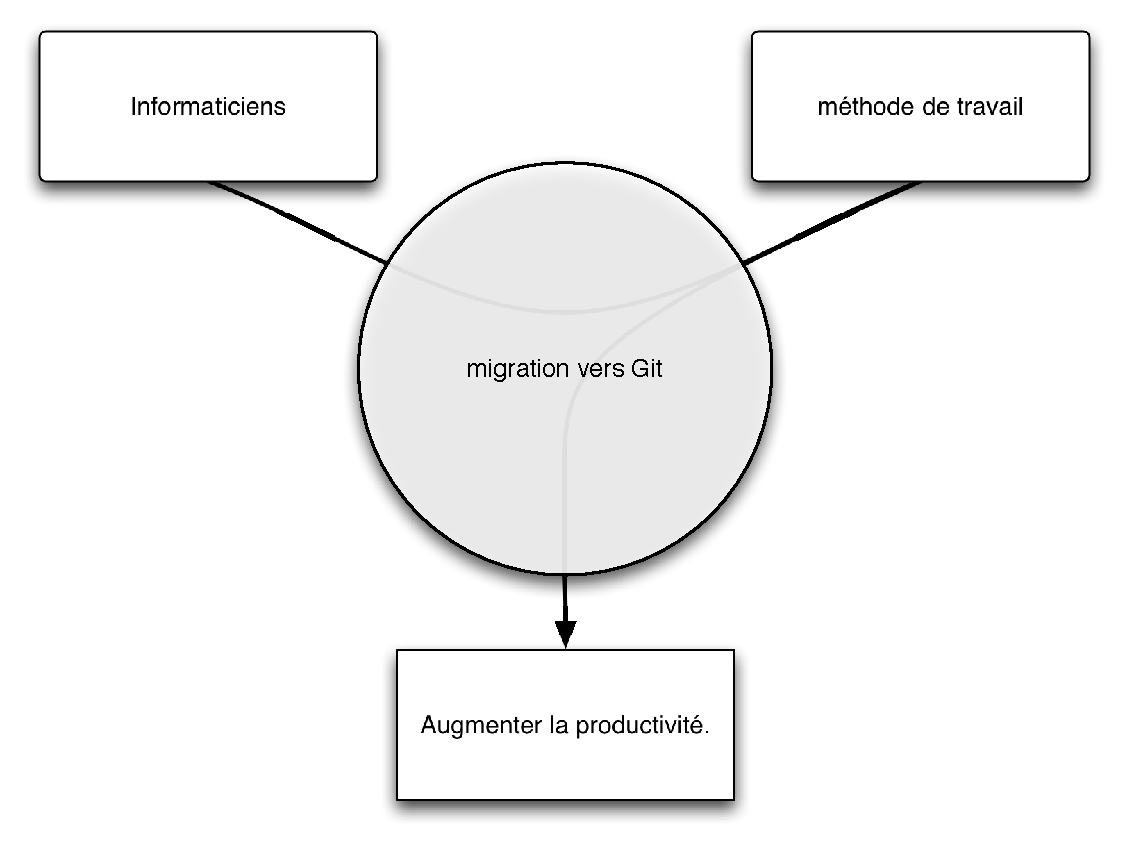
\includegraphics[width=0.95\textwidth]{pictures/GitBAC}
\end{center}
\caption{Bête à cornes (méthode {APTE\textregistered}) de la migration vers Git}
\label{fig:BACGit}
\end{figure}

{\gofigure} est un projet qui prend de l'ampleur,
nous souhaitons remplacer SVN par Git pour les multiples avantages
que ce dernier apporte à la gestion du projet et ainsi améliorer le protocole de travail.

La migration vers Git provient d'un besoin exprimé par la communauté de développeurs libres principalement.
Il permettra à l'équipe de {\gofigure} de travailler 
avec un nouveau standard de développement en suivant un workflow précis, qui facilite le travail en équipe.

Cette migration a été repoussée jusqu'à ce que Git soit adopté comme standard dans les communautés de développeurs.
Il est important de proposer un protocole de travail qui soit assez flexible pour permettre à l'équipe de le suivre,
tout au long de l'évolution de {\gofigure}.
L'information donnée à l'équipe informatique devra évoluer en même temps que Git, et que le projet {\gofigure}.


\subsubsection*{Diagramme pieuvre de la migration vers Git}

\begin{figure}[h]
\begin{center}
\leavevmode
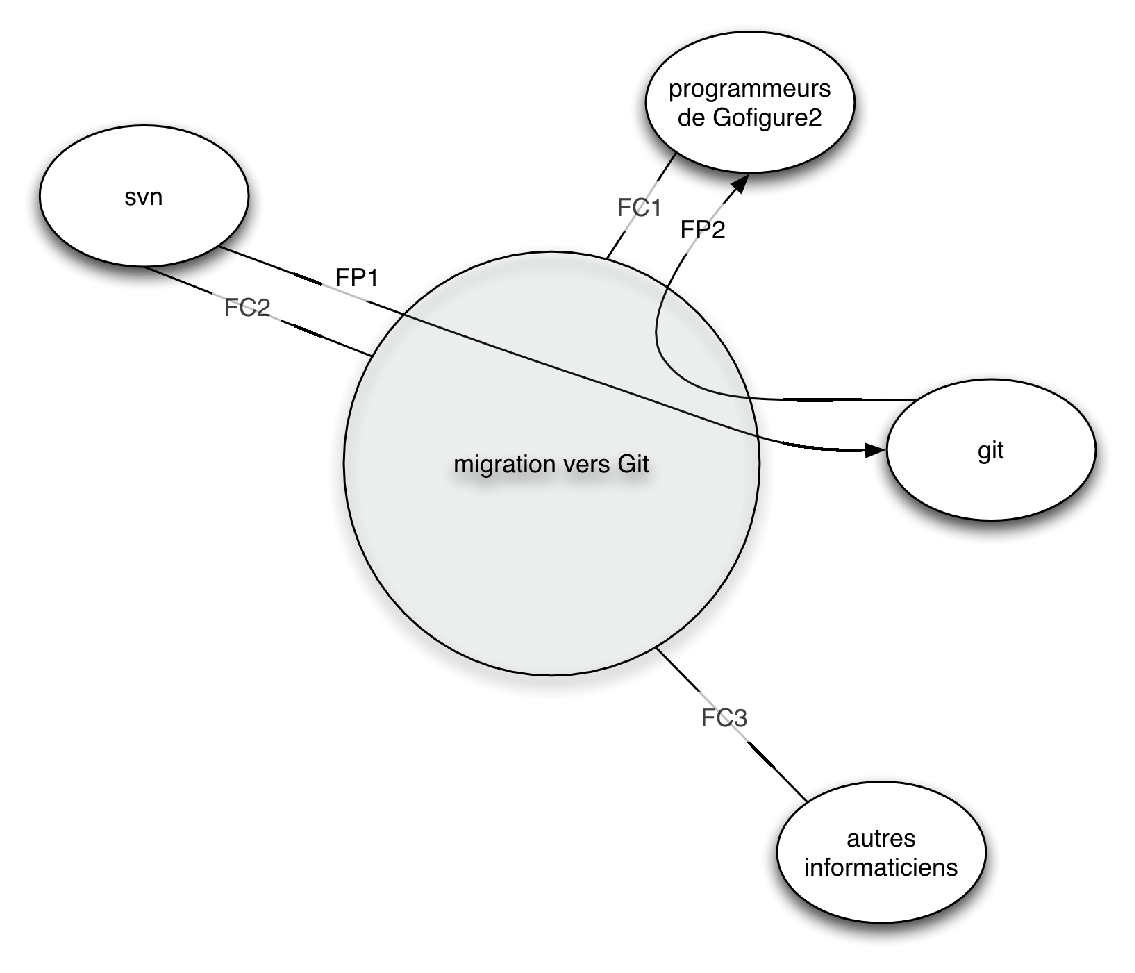
\includegraphics[width=0.95\textwidth]{pictures/GitPIEUVRE}
\end{center}
\caption[Diagramme Pieuvre (méthode {APTE\textregistered}) de la migration vers Git]{Diagramme Pieuvre (méthode {APTE\textregistered}) de la migration vers Git

\small
\textbf{Fonctions principales :}\\
FP1 : migrer le projet {\gofigure} de SVN à Git.\\
FP2 : proposer un workflow aux programmeurs de l'équipe de {\gofigure}.\\
\textbf{Fonctions contraintes :} \\
FC1 : apporter une base de connaissance sur Git aux programmeurs de {\gofigure}.\\
FC2 : rester compatible avec SVN.{\gofigure}
FC3 : donner la possibilité à d'autres informaticiens de participer au projet.}
\label{fig:PIEUVREGit}
\end{figure}

\clearpage

Voici l'analyse du {\gofigure} pieuvre du projet de migration de {\gofigure} vers Git :

\paragraph*{FP1} : migrer le projet {\gofigure} de SVN à git.
\begin{itemize}
  \item Existe pour améliorer le travail collaboratif sur {\gofigure}.
  \item Existe à cause de l'apparition de nouveaux programmes performant combinant la gestion et la distribution de sources.
  \item Pourrait disparaitre si un nouveau modèle plus performant et intéressant pour l'équipe de {\gofigure} venait à apparaitre.
  Si la nouvelle version de SVN était adoptée par la communauté des développeurs libres.
\end{itemize}

\paragraph*{FP2} : proposer un workflow aux programmeurs de l'équipe de {\gofigure}.
\begin{itemize}
  \item Existe pour structurer le travail avec Git.
  \item Existe du fait de l'extrême souplesse de Git : ce programme 
  permet de créer pratiquement n'importe quelle architecture de développement.
  \item Pourrait évoluer après une période d'étalonnage pour vérifier la pertinence du protocole.
  Si une norme venait à apparaitre.
\end{itemize}

\paragraph*{FC1} : apporter une base de connaissance sur Git aux programmeurs de {\gofigure}.
\begin{itemize}
  \item Existe pour permettre aux programmeurs d'utiliser Git.
  \item Existe car Git est relativement complexe à prendre en main 
  pour un utilisateur habitué à d'autres programmes de gestion de source centralisés comme SVN.
  \item Pourrait disparaitre en partie si Git devenait trivial à l'usage.
  Il est important qu'une telle aide évolue avec Git, et avec le workflow de {\gofigure}.
\end{itemize}

\paragraph*{FC2} : rester compatible avec SVN.
\begin{itemize}
  \item Existe pour permettre a un programmeur de continuer à utiliser SVN, et migrer vers Git progressivement.
  Existe aussi pour ouvrir les sources de {\gofigure} à plus de développeurs potentiels.
  \item Existe car tous les programmeurs n'utilisent pas (encore) Git.
  \item Pourrait disparaitre si SVN disparaissait.
\end{itemize}

\paragraph*{FC3} : donner la possibilité à d'autres informaticiens de participer au projet.
\begin{itemize}
  \item Existe pour permettre a un maximum de programmeur de télécharger {\gofigure}, l'utiliser et participer à son développement.
  \item Existe car la librairie est open-source et s'améliore avec les contributions d'autres utilisateurs.
  \item Pourrait disparaitre si le protocole de travail n'était pas adapté à l'adjonction de code produit par un développeur tierce.
\end{itemize}


\subsection{Résultats}

\subsubsection{Écriture du tutoriel}

Le tutoriel a été écrit sur le wiki de {\gofigure}. Il s'agit de l'emplacement de prédilection pour les informations 
concernant la programmation et l'utilisation de {\gofigure}. Le système du wiki, en plus de proposer une syntaxe simple 
pour créer des pages web formatées, permet aux lecteurs autorisés de modifier le contenu. 
Il existe aussi un système de feedback permettant aux lecteurs ayant mal compris le contenu, de contacter l'auteur.

Ce tutoriel remplit les fonction FC1 et FC3, présentées dans le diagramme Pieuvre(figure~\ref{fig:PIEUVREGit})

L'écriture d'un tel tutoriel se fait souvent dans un registre proche du langage familier,
le but étant de simuler des instruction données par un collègue ou un ami. 
Les instructions se doivent d'être relativement brèves, bien souvent le lecteur veut juste appliquer certaines fonctionnalités 
proposées par Git sans toujours vraiment chercher à comprendre ce qu'il fait. 
Il existe d'autres sources d'informations pour apprendre complètement le fonctionnement de l'application.
Le tutoriel ne se veut donc pas exhaustif, il propose juste une manière qui fonctionne d'utiliser Git,
à la manière d'un travail dirigé. Il a été écrit pendant ma phase d'apprentissage de Git. 
Il détaille les principales difficultés et écueils rencontrés. 

Le tutoriel est présent à cette adresse : \\
\url{http://sourceforge.net/apps/trac/gofigure2/wiki/GIT}

\subsubsection{Proposition d'un protocole de travail}
Il a enfin fallu proposer un workflow (protocole de travail) 
qui définit la manière dont les programmeurs
doivent apporter des modifications au code source.
Afin de répondre aux fonctions FP2, FC2 et FC3 du diagramme pieuvre du cahier des charges, il fallait proposer un protocole qui :
\begin{enumerate}
  \item n'augmente pas trop la charge de travail,
  \item permette de bien suivre les modifications apportées par chacun. 
  \item permette au responsable du projet de corriger ou supprimer les changements apportés par les développeurs.
  \item corresponde à un standard.
\end{enumerate}

Le workflow proposé a été détaillé par \href{http://nvie.com/about }{Vincent Driessen} sur son \href{http://nvie.com/Git-model}{blog}.
Ce protocole découle assez naturellement de l'apprentissage de Git, il est donc simple.

\begin{figure}[h]
\begin{center}
\leavevmode
\includegraphics[width=0.95\textwidth]{pictures/Git_WorkflowSimple}
\end{center}
\caption{Diagramme simplifié du workflow proposé pour l'équipe de gofigure}
\label{fig:WorkflowGitSimple}
\end{figure}

Ce workflow, en plus d'être précisément détaillé, est techniquement viable. 
Voici le détail de l'organisation du projet {\gofigure} sous ce protocole.

Il existe deux branches principales : 
\begin{description}
  \item[\emph{master}] : cette branche stocke les versions stables du programme.
  \item[\emph{develop}] : cette branche contient la dernière version commune du programme, elle correspond au tronc.
\end{description}
Ces branches sont présentes sur le serveur central. Le développement du programme se fait sur la branche \emph{develop}, et lorsqu'une version stable est sur le point d'être produite, on sauvegarde l'état d'avancement du projet dans la branche \emph{master}.

Il existe ensuite une série de branches de support.
Ces branches ont une durée de vie limitée, et doivent fusionner avec d'autres branches pour finalement rejoindre \emph{develop} (le tronc), puis \emph{master}.
Elles ne sont pas forcément présentes sur le serveur central, cela dépend des équipes travaillant sur les différentes parties du programme.
\begin{description}
  \item[\emph{feature}] : cette branche contient le développement d'une fonction du programme. Elle est créée à partir de \emph{develop}, et une fois mature, refusionne avec \emph{develop}.
  \item[\emph{release}] : cette branche permet aux développeurs de travailler sur la correction de bugs, l'interface graphique, l'ajout de tests... les touches de dernière minute, avant la publication d'une nouvelle version du programme. Elle est créée lorsque la branche \emph{develop} contient toutes les fonctions attendues pour la nouvelle version du programme. Elle est créée à partir de la branche \emph{develop} et une foi mature, fusionne avec la branche \emph{master}, et \emph{develop}.
  \item[\emph{hotfixes}] : cette branche particulière est créée à partir de la branche \emph{master}, lorsqu'une version publiée du programme contient un bug important qui ne peut attendre la prochaine version pour être corrigée. Elle refusionne avec la branche \emph{master} pour créer des "sous versions" (0.1.1 par exemple, est une sous version de 0.1.0). Cette branche particulière merge aussi avec la branche \emph{develop} pour appliquer la correction aux futures publications, et enfin, la branche \emph{release} si elle existe au moment de la réparation du bug.
\end{description}

Un cycle de développement simplifié est illustré figure~\ref{fig:WorkflowGitSimple}.
Il est important de noter que bien souvent, les informaticiens travaillent sur plusieurs choses à la fois,
et ce workflow permet ce genre d'organisation. 

\subsubsection{Mise en œuvre de la Migration vers Git}

Maintenant le workflow défini, et l'aide mise en place, il faut mettre en œuvre la migration vers Git du projet afin de répondre à FP1 de la figure~\ref{fig:PIEUVREGit}. Nous devons choisir une plateforme pour héberger le projet, et mettre en place des liens entre le serveur SVN et le serveur Git.

\subsubsection*{Github : une plateforme de travail collaboratif}

\href{https://github.com/}{Github} propose d'héberger gratuitement les projets open-sources. Les serveurs github sont administrables par un site
internet : \url{http://github.com/}. L'originalité de l'interface réside dans le réseau social proposé par le site. Il est possible de consulter les profils des programmeurs, de voir en temps réel l'avancement des projets sur lesquels ils travaillent. Le "fork" (copie d'un projet open source en vue de le modifier/l'améliorer) se fait en un click. Les collaborations se mettent en place d'une manière totalement transparente.
\begin{figure}[h]
\begin{center}
\leavevmode
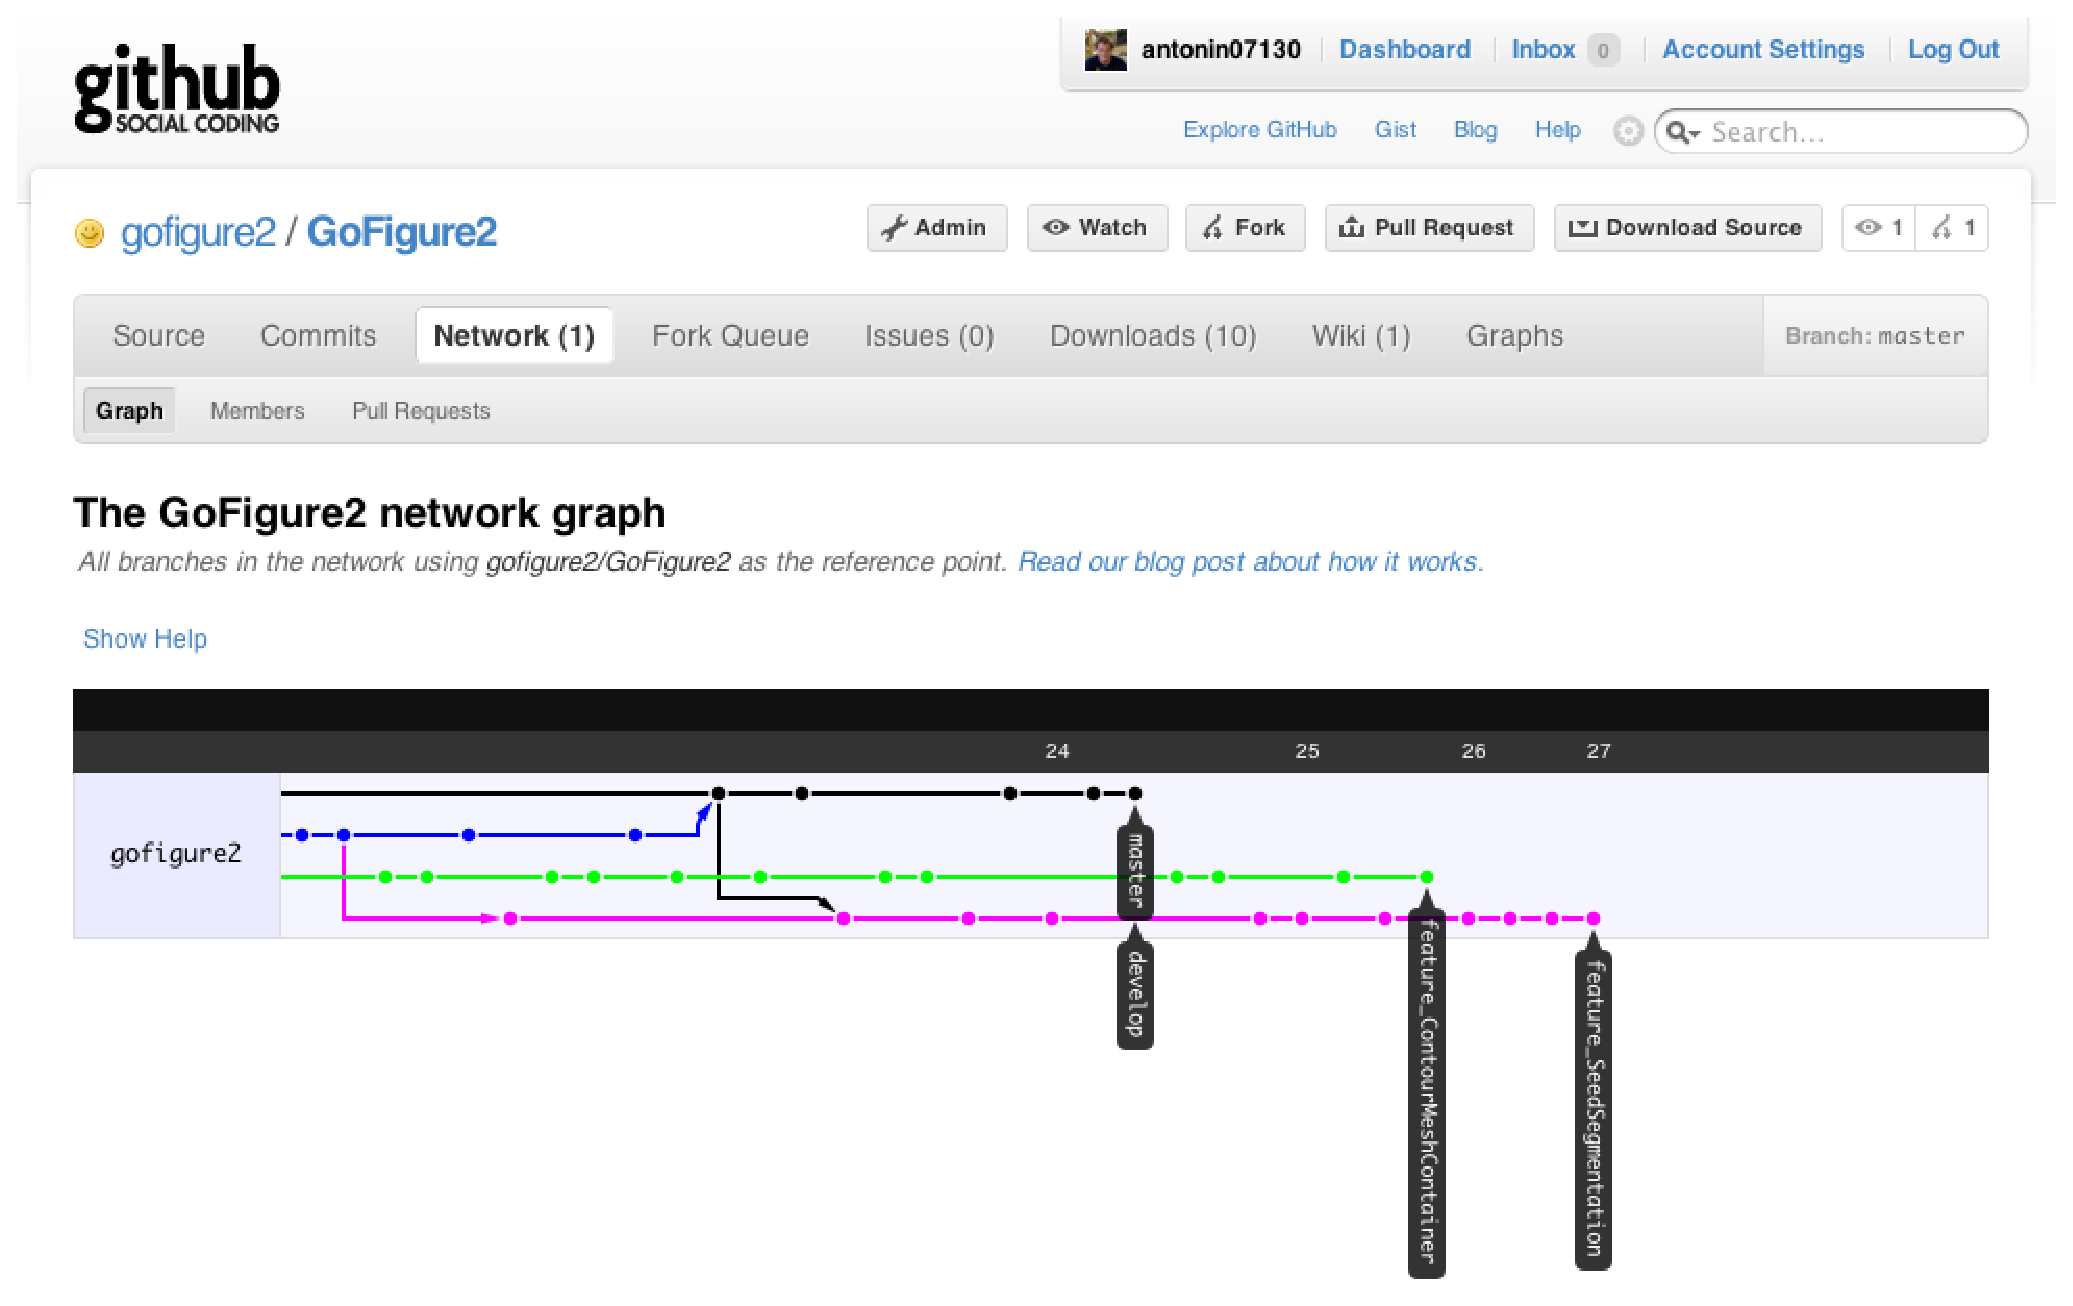
\includegraphics[width=0.95\textwidth]{pictures/GitGithub}
\end{center}
\caption{Network de Gofigure2 sur Github. Les points représentent des commits. Les branches sont clairement visibles.}
\label{fig:GitGithub}
\end{figure}
Nous avons donc opté pour cette plateforme, qui est une autre raison de la montée de Git comme programme de gestion de sources. Les connections sur ce site sont sécurisées par un protocole crypté (ssh)... Il est donc nécessaire d'effectuer certaines opérations de configuration avant de pouvoir utiliser les serveurs Git de Github. Les détails de la création d'un compte ont été repris dans le tutoriel à destination de l'équipe de {\gofigure}.

\subsubsection*{Automatisation de la migration vers Git}

Une fois l'organisation {\gofigure} créée sur Github, et les comptes des développeurs configurés, nous avons pu passer à la migration à proprement parler du projet.
Nous avons ensuite copié le contenu du serveur SVN de {\gofigure},
pour le traduire en un projet Git, en respectant le workflow proposé.

La figure~\ref{fig:MigrationGit} schématise la mise à jour du serveur Git avec les informations du serveur SVN.
Pour l'instant cette synchronisation est journalière. Le script correspondant est donné en annexe~\ref{AnnexeScriptGIT}. L'exécution de ce dernier est planifiée grâce à l'utilitaire "cron" (paramétrable avec "cronjob"), présent sur les plateformes unix.
Nous pourrions aussi envisager une mise à jour automatique à chaque modification du projet.
Un cycle de développement simplifié devient donc, pour un programmeur :

Le serveur du Megason Lab copie donc tous les jours les informations du serveur SVN.
Il transforme ces informations pour qu'elles soient compatibles avec le protocole de Git,
et conforme au protocole de travail proposé, puis les envoie sur le serveur de github.
Pour l'instant, les modifications provenant du serveur de Github (flèches pointillées)
sont manuellement intégrées au projet. Cependant, on peut facilement automatiser cette fusion des projets Git et SVN.
La figure~\ref{fig:GitGithub} montre le projet {\gofigure} sur Github. L'importation de ce projet a été automatiquement résolue par le script montré en annexe~\ref{AnnexeScriptGIT}.

\begin{figure}[h]
\begin{center}
\leavevmode
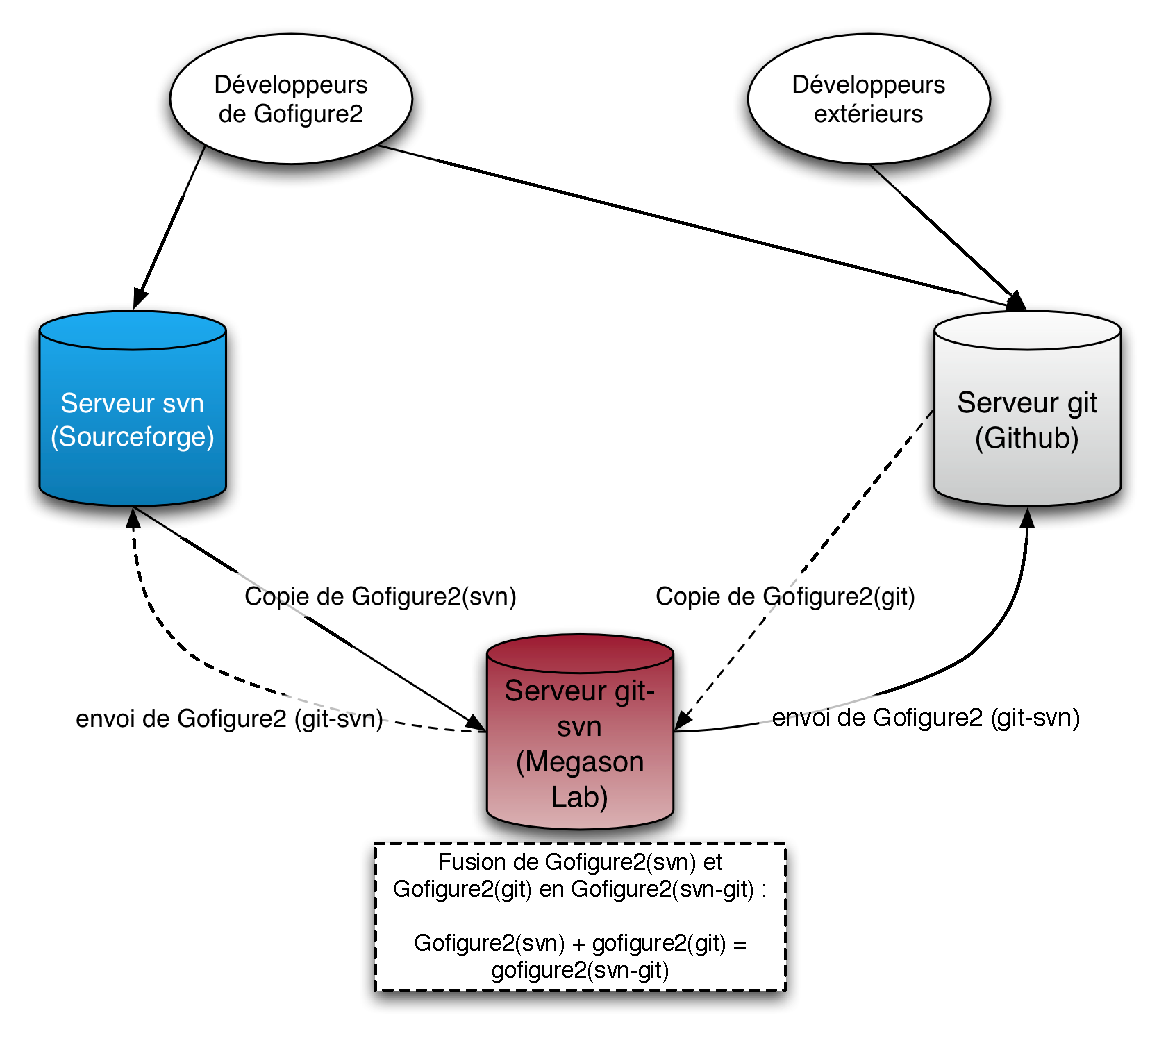
\includegraphics[width=0.95\textwidth]{pictures/GitTransfert}
\end{center}
\caption{Migration automatique de SVN vers Git via un serveur installé au Megason Lab}
\label{fig:MigrationGit}
\end{figure}

\clearpage

\subsubsection*{Conclusion}

\paragraph*{}
Ce projet a encore une fois été extrêmement instructif.
Il m'a permis de m'intéresser à la gestion de version et des outils existants pour cela.
On se rend vite compte que ces programmes très performants vont bien plus loin que simplement archiver les modifications des projets.
Ils permettent réellement de manager un projet en forçant une démarche de travail, et en gardant trace des modifications apportées par chacun.
De plus Github a réellement transformé la manière de programmer en introduisant l'aspect réseau social dans les projets.

\paragraph*{}
Ce projet comportait bien-sûr des difficultés, notamment l'apprentissage de Git. Ce programme est très puissant et flexible, de fait, il est possible de faire la même chose de plusieurs manières. Différencier la "bonne" et la "mauvaise" façon de travailler peut être difficile. Cela s'est fait ressentir lors de l'écriture du tutoriel : au fur et à mesure que j'apprenais Git, je réécrivais des chapitres, afin de les simplifier.

Il existe de nombreuses ressources sur internet, chacune proposant une utilisation du programme.
Git est aussi totalement différent des programmes de gestion de versions centralisés. Cela bouleverse les habitudes que l'on peut avoir en utilisant SVN par exemple.

Enfin, le choix d'un workflow n'est pas toujours évident, il faut savoir anticiper le futur de {\gofigure}, et choisir un protocole bien structuré. 

La migration a été assez facile comme je maitrisais alors bien Git. Quelques difficultés liées à cronjob, et aux droits d'utilisateur pour les connections sécurisées sous unix sont apparues.




%--------------------------------------------------
%             RECALAGE
%--------------------------------------------------

\section{Amélioration des techniques d'imagerie}

Ce projet part d'une initiative personnelle : ayant appris qu'il m'était possible de continuer à travailler au Megason Lab, sur des images acquises par le microscope confocal, je décidai d'améliorer la qualité des images acquises. En effet, ces données formeront la base de mes futures recherches, et trouver un moyen de les améliorer faciliterait d'autant mon travail.

Je me suis penché sur un problème très courant dans ce type d'imagerie : 
celui du mouvement incontrôlé du spécimen.
Les poissons zèbre sont insérés manuellement dans des supports créés spécialement par le Megason Lab (figuresı\ref{fig:PICMounting}~et~\ref{fig:PICMount}). Ces supports permettent aux poissons de grandir tout en les gardant dans une position statique. Cependant, ils ne peuvent restreindre totalement les mouvements des spécimens.

Cela a des conséquences catastrophiques sur la qualité des images : 
la région étudiée du spécimen peut être en dehors 
du champ microscopique\footnote{Un champ microscopique ou champ d'observation est la zone d'observation éclairée qui apparait au manipulateur lors d'une observation au microscope}
après quelques heures d'acquisition,
cela conduit aussi à des "sauts" violents causés par la remise en place manuelle de l'objectif.

Je vais tout d'abord prouver la validité d'un tel projet (projet de recalage), pour ensuite détailler la réalisation technique qu'il a engendrée.
\begin{figure}[h]
\begin{center}
\leavevmode
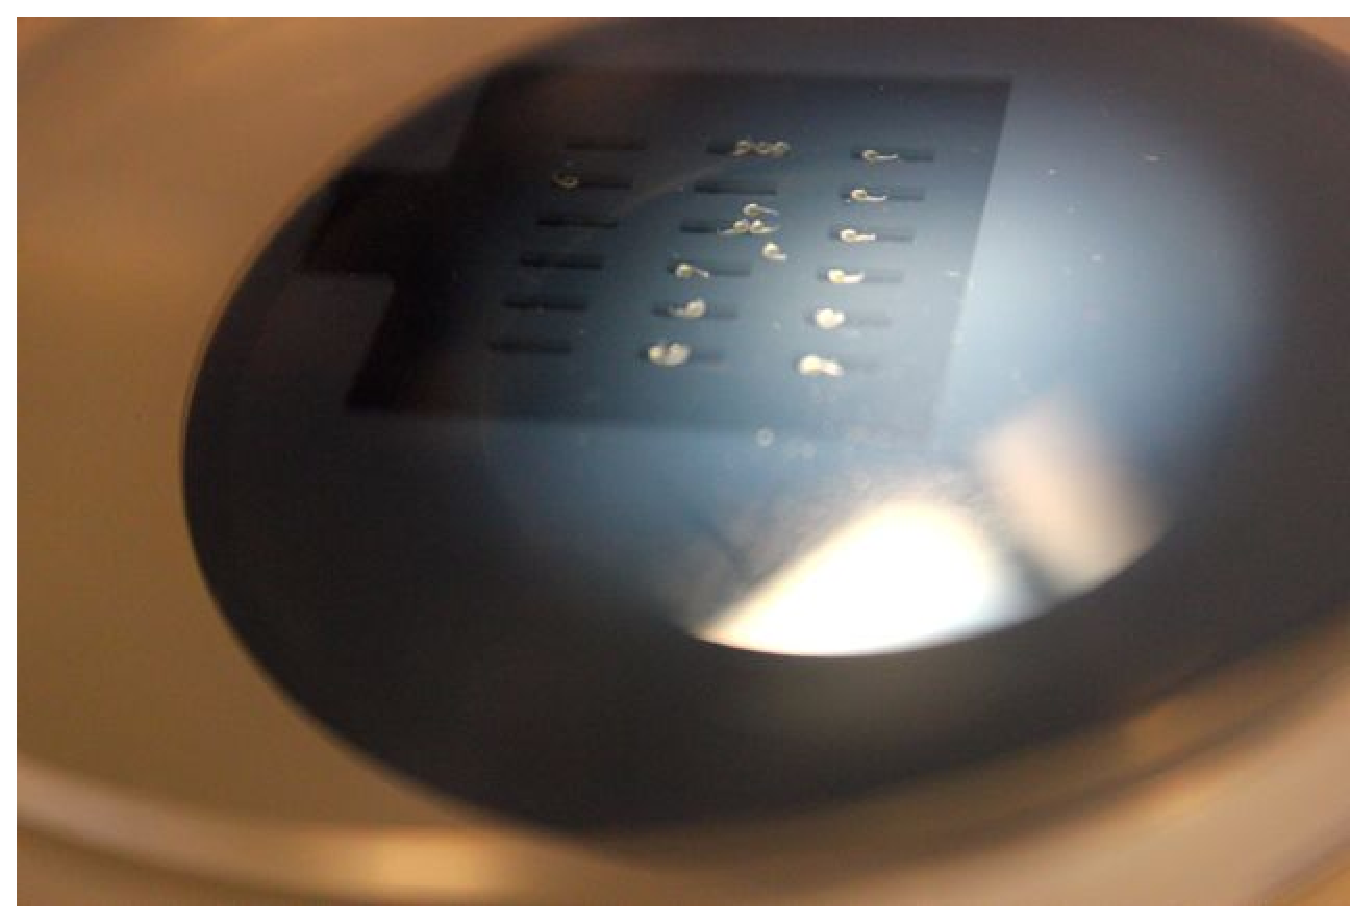
\includegraphics[width=0.95\textwidth]{pictures/PICmount}
\end{center}
\caption{Les supports d'embryons de poissons zèbres, spécialement créés au Meagson Lab pour permettre d'imager les spécimens pendant leur croissance.}
\label{fig:PICMount}
\end{figure}

\begin{figure}[h]
\begin{center}
\leavevmode
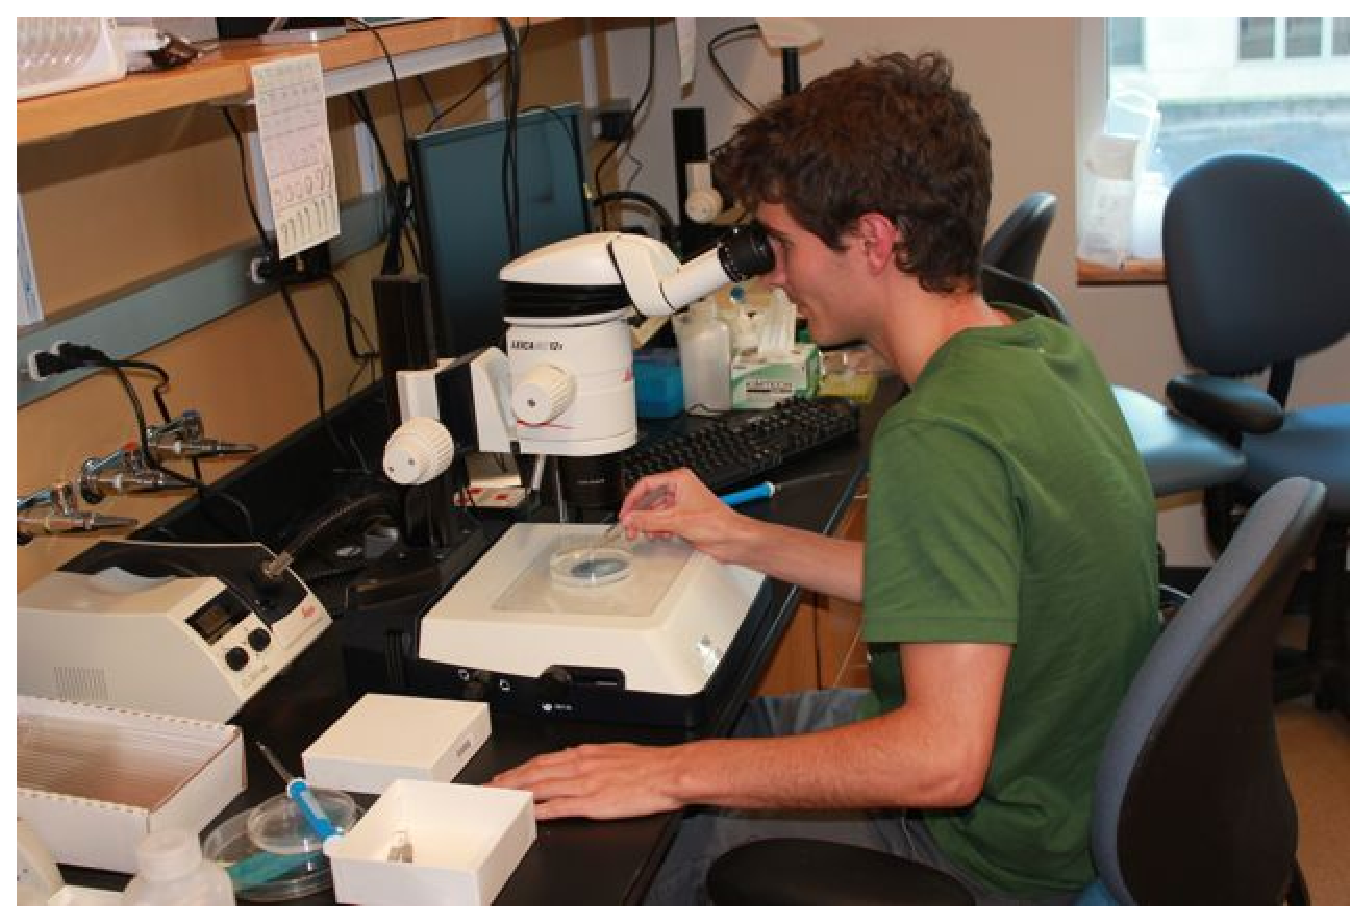
\includegraphics[width=0.95\textwidth]{pictures/PICmounting}
\end{center}
\caption{Un biologiste en train d'insérer manuellement les embryons de poissons zèbre dans un support, en vue de les imager.}
\label{fig:PICMounting}
\end{figure}

\subsection{Cahier des charges}
Nous commençons par présenter la Bête à Cornes,
pour clarifier le but principal du projet. Nous présentons ensuite le diagramme pieuvre qui permet de détailler les fonctions du projet.

\subsubsection{Contrôle de la validité du projet}
\begin{figure}[h]
\begin{center}
\leavevmode
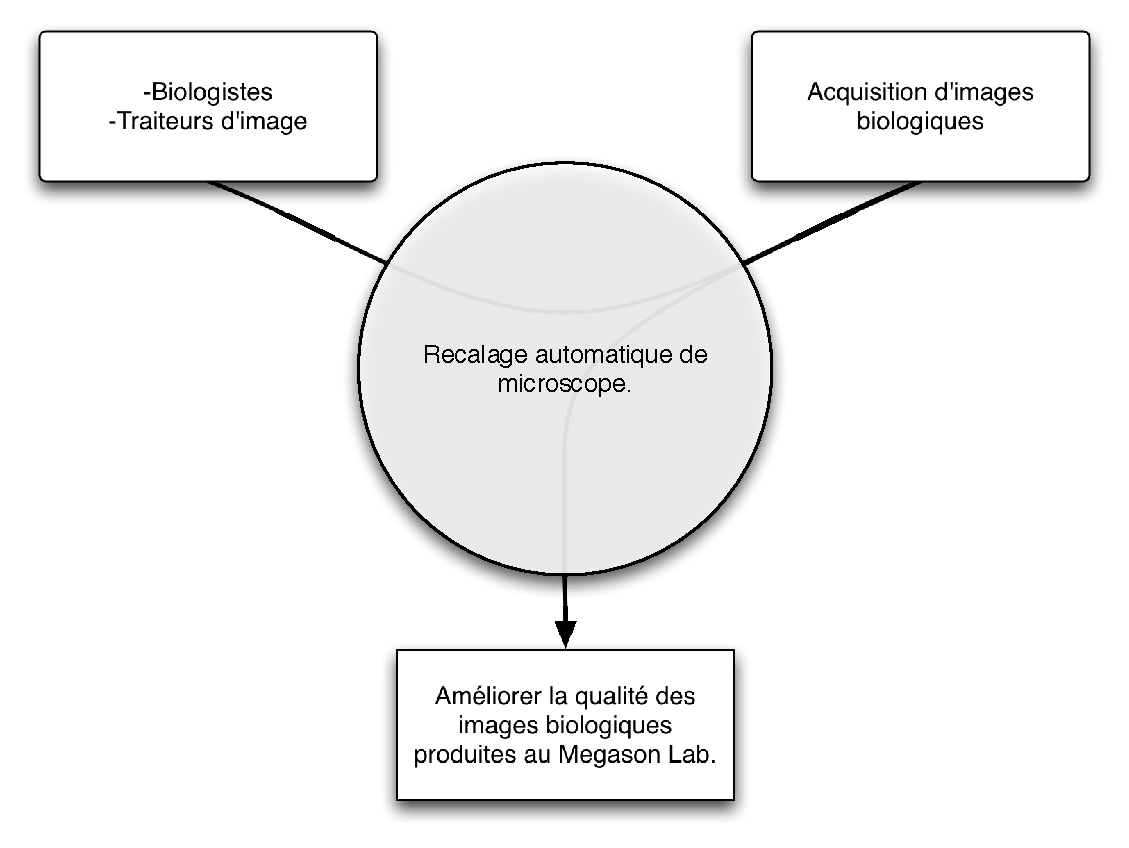
\includegraphics[width=0.95\textwidth]{pictures/RecalBAC}
\end{center}
\caption{Bête à cornes (méthode {APTE\textregistered}) du projet de suivi de spécimen}
\label{fig:BACRecal}
\end{figure}

La figure~\ref{fig:BACRecal} montre la Bête à cornes du projet de recalage d'images microscopiques.

La réalisation de ce produit résulte d'un besoin exprimé par les biologistes et traiteurs d'images.
Comme le spécimen change de forme durant la phase d'imagerie, il arrive qu'il ne soit plus dans le champ d'observation, ce qui est un réel problème pour les biologistes qui doivent contrôler l'alignement du microscope toutes les heures.
C'est aussi un problème pour les traiteurs d'images
car il arrive qu'un biologiste déplace en un mouvement un spécimen.
Cela invalide beaucoup de méthodes de suivi des objets imagés.

Ce projet, en automatisant l'alignement du microscope permet donc aux biologistes de moins surveiller l'acquisition,
et aux traiteurs d'images, de disposer de données exploitables.

Ce projet peut évoluer en accord avec les besoins des biologistes, et suivant l'évolution des techniques de recalage d'images.

\subsubsection{Expression fonctionnelle}

\begin{figure}[h]
\begin{center}
%\leavevmode
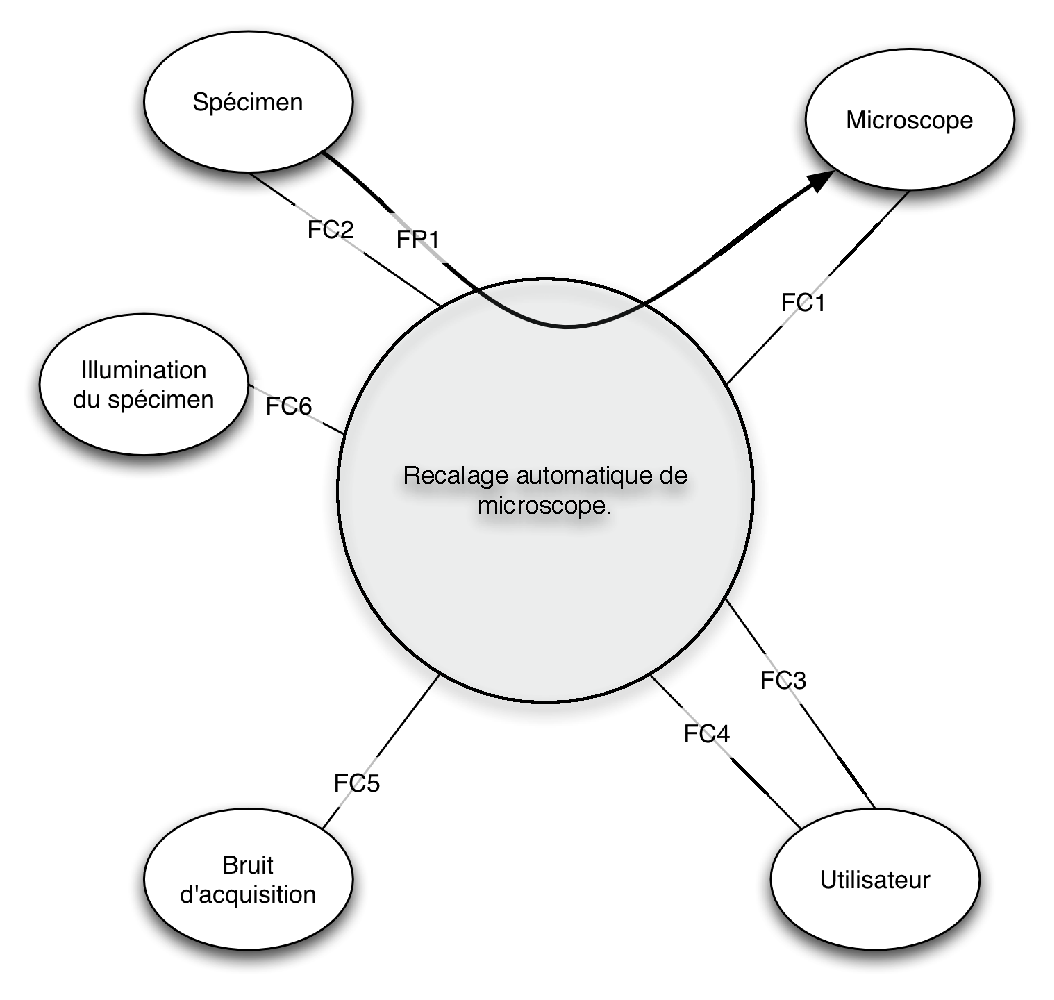
\includegraphics[width=0.9\textwidth]{pictures/RecalPIEUVRE}
\end{center}
\caption[Diagramme Pieuvre (méthode {APTE\textregistered}) du projet de suivi de spécimen]{Diagramme Pieuvre (méthode {APTE\textregistered}) du projet de suivi de spécimen

\small
\textbf{Fonction principale :}\\
FP1 : déplacer le microscope pendant l'acquisition en suivant le spécimen\\
\textbf{Fonctions contraintes :} \\
FC1 : compatible avec les logiciels utilisés\\
FC2 : robuste aux changements de forme du spécimen\\
FC3 : contenir une interface homme machine\\
FC4 : maintenable par l'équipe du Megason Lab\\
FC5 : robuste au bruit\\
FC6 : robuste aux changements d'illumination\\
FC7 : rapide}
\label{fig:PIEUVRERecal}
\end{figure}

\clearpage

La figure~\ref{fig:PIEUVRERecal} est le diagramme pieuvre du projet, que nous analysons :

\paragraph*{FP1} : déplacer le microscope pendant l'acquisition en suivant le spécimen.
\begin{itemize}
  \item Existe pour créer des images exploitables d'une manière fiable.
  \item Existe à cause de la nature du spécimen analysé, qui est vivant et en développement. 
  Il change donc de forme, grossit et se déplace, il faut donc suivre l'organe d'intérêt pendant le
  développement du spécimen.
  \item Pourrait disparaitre si le Megason Lab arrêtait d'imager des spécimens vivants.
  Si les microscopes avaient un champ de visualisation assez grand pour englober
  tout le spécimen et d'éventuelles marges de déplacement.
\end{itemize}

\paragraph*{FC1} : compatible avec les logiciels utilisés.
\begin{itemize}
  \item Existe pour fonctionner avec le matériel présent au Megason Lab.
  \item Existe à cause de la nature des logiciels utilisés au Megason Lab.
  \item Pourrait disparaitre si le logiciel de contrôle du Megason Lab était compatible avec n'importe quel langage informatique,
  en particulier le {\C++}.
\end{itemize}

\paragraph*{FC2} : robuste aux changements de forme du spécimen
\begin{itemize}
  \item Existe pour fonctionner sur différents spécimens analysés,
  et sur une période de temps étendue (le spécimen change de forme au cours du temps).
  \item Existe à cause de la nature des spécimens analysés au Megason Lab.
  \item Pourrait disparaitre si les spécimens n'évoluaient pas au cours du temps;
  si il existait un programme spécifique à chaque partie du spécimen.
\end{itemize}

\paragraph*{FC3} : contenir une interface homme machine
\begin{itemize}
  \item Existe pour interagir avec l'utilisateur.
  \item Existe à cause du besoin du programme de paramètres provenant de l'utilisateur.
  \item Pourrait disparaitre si le programme pouvait déterminer automatiquement les meilleurs paramètres.
\end{itemize}

\paragraph*{FC4} : maintenable par l'équipe du Megason Lab
\begin{itemize}
  \item Existe pour permettre aux autres chercheurs du Megason Lab de modifier/utiliser le programme.
  \item Existe car le développeur de l'application ne sera pas toujours présent pour la maintenir.
  \item Pourrait disparaitre si le programme se maintenait tout seul.
\end{itemize}

\paragraph*{FC5} : robuste au bruit
\begin{itemize}
  \item Existe pour permettre à l'algorithme de fonctionner en la présence de bruit
  \item Existe car le microscope produit des images bruitées.
  \item Pourrait disparaitre si le microscope produisait des images sans aucun bruit.
\end{itemize}


\paragraph*{FC6} : robuste aux changement d'illumination
\begin{itemize}
  \item Existe pour permettre à l'algorithme de fonctionner au cours du temps. 
  \item Existe car la fluorescence des spécimens décroit au cours du temps (phénomène de "bleaching"),
  et change d'une image à l'autre car le système d'illumination basé sur une probabilité d'absorption de photons.
  (le même phosphore n'absorbe pas toujours autant de photons avant de ré-émettre).
  \item Pourrait disparaitre si le bleaching disparaissait 
  et si nous contrôlions mieux l'absorption de photons par les phosphores du spécimen.
\end{itemize}

\paragraph*{FC7} : rapide
\begin{itemize}
  \item Existe pour permettre au microscope de faire des acquisitions peu espacées dans le temps
  \item Existe car l'alignement du microscope doit être fait avant l'acquisition.
  \item Pourrait disparaitre ou évoluer si nous intégrions une prédiction
  des déplacements futurs en fonction des déplacements précédents.
\end{itemize}

\subsection{Solutions techniques}

Le principe du programme est d'estimer le déplacement de structures notables dans l'image.
Une fois ce déplacement estimé, il s'agit de déplacer le spécimen afin de garder ces structures dans le champ du microscope.

\subsubsection{Estimation du déplacement du spécimen}
Nous utilisons le principe du recalage d'images
\footnote{Le recalage d'images est une technique utilisée en traitement d'image pour mettre en correspondance les informations
provenant de deux images différentes. Afin d'aligner les images, une transformation géométrique est recherchée.
Cette transformation est choisie de manière à minimiser un critère de différence entre les images.
Le choix de la transformation et du critère de différence sont donc primordiaux.}
 pour estimer le déplacement du spécimen entre deux acquisitions (deux images) effectuées par le microscope : si nous trouvons une translation qui permette de passer d'une acquisition à l'autre, nous pouvons estimer le déplacement du spécimen.
Comme le microscope ne peut que déplacer le spécimen en translation, nous choisissons un recalage rigide qui évalue les translations selon les trois dimensions de l'espace, entre deux images 3D.

Les techniques de recalage sont basées sur des critères de différence à minimiser.
On choisit ces critères de manière à ce que leur valeur soit élevée quand deux images sont mal alignées,
et faibles quand elles sont alignées. Notre programme teste différentes translations jusqu'à trouver une translation
qui donne une faible valeur du critère d'énergie.
Bien sûr, il n'est pas possible de calculer le critère de différence pour toute les translations possibles car cela prendrait trop de temps.
On choisit donc une technique qui "dirige" les estimations de manière à diminuer l'énergie
(la descente de gradient est une technique classique).
Enfin, afin que notre algorithme soit robuste vis à vis du bruit, et des changements de forme peu significatifs,
nous moyennons les images, puis réduisons la résolution des images moyennées.
Le facteur de réduction dépend de la taille du spécimen, des structures à analyser,
et de la résolution initiale des images acquises par le microscope.

Le choix de la métrique est basé sur plusieurs critères : la simplicité d'utilisation (peu de paramètres),
la robustesse au bruit et aux changements d'illumination, et la robustesse aux changements de forme. Il faut enfin que cet algorithme soit rapide : le déplacement est calculé entre chaque acquisition, et doit prendre moins d'une minute au total. Ce choix est donc dicté par les contraintes FC2 à FC7 du diagramme pieuvre (figure\ref{fig:PIEUVRERecal}) !

Afin de sélectionner une métrique, plusieurs essais ont étés effectués, tout d'abord avec des déplacements simulés,
puis avec de réelles séquences d'images microscopiques. Les métriques évaluées sont : le critère de corrélation normalisé (décrit dans\cite{registrationCrossCorr}), le critère d'information mutuelle de Mattes (décrit dans \cite{mattes2001nonrigid}), et le critère de la différence entre pixels élevée au carré (les "moindres carrés").

\begin{figure}[h]
\begin{center}
\leavevmode
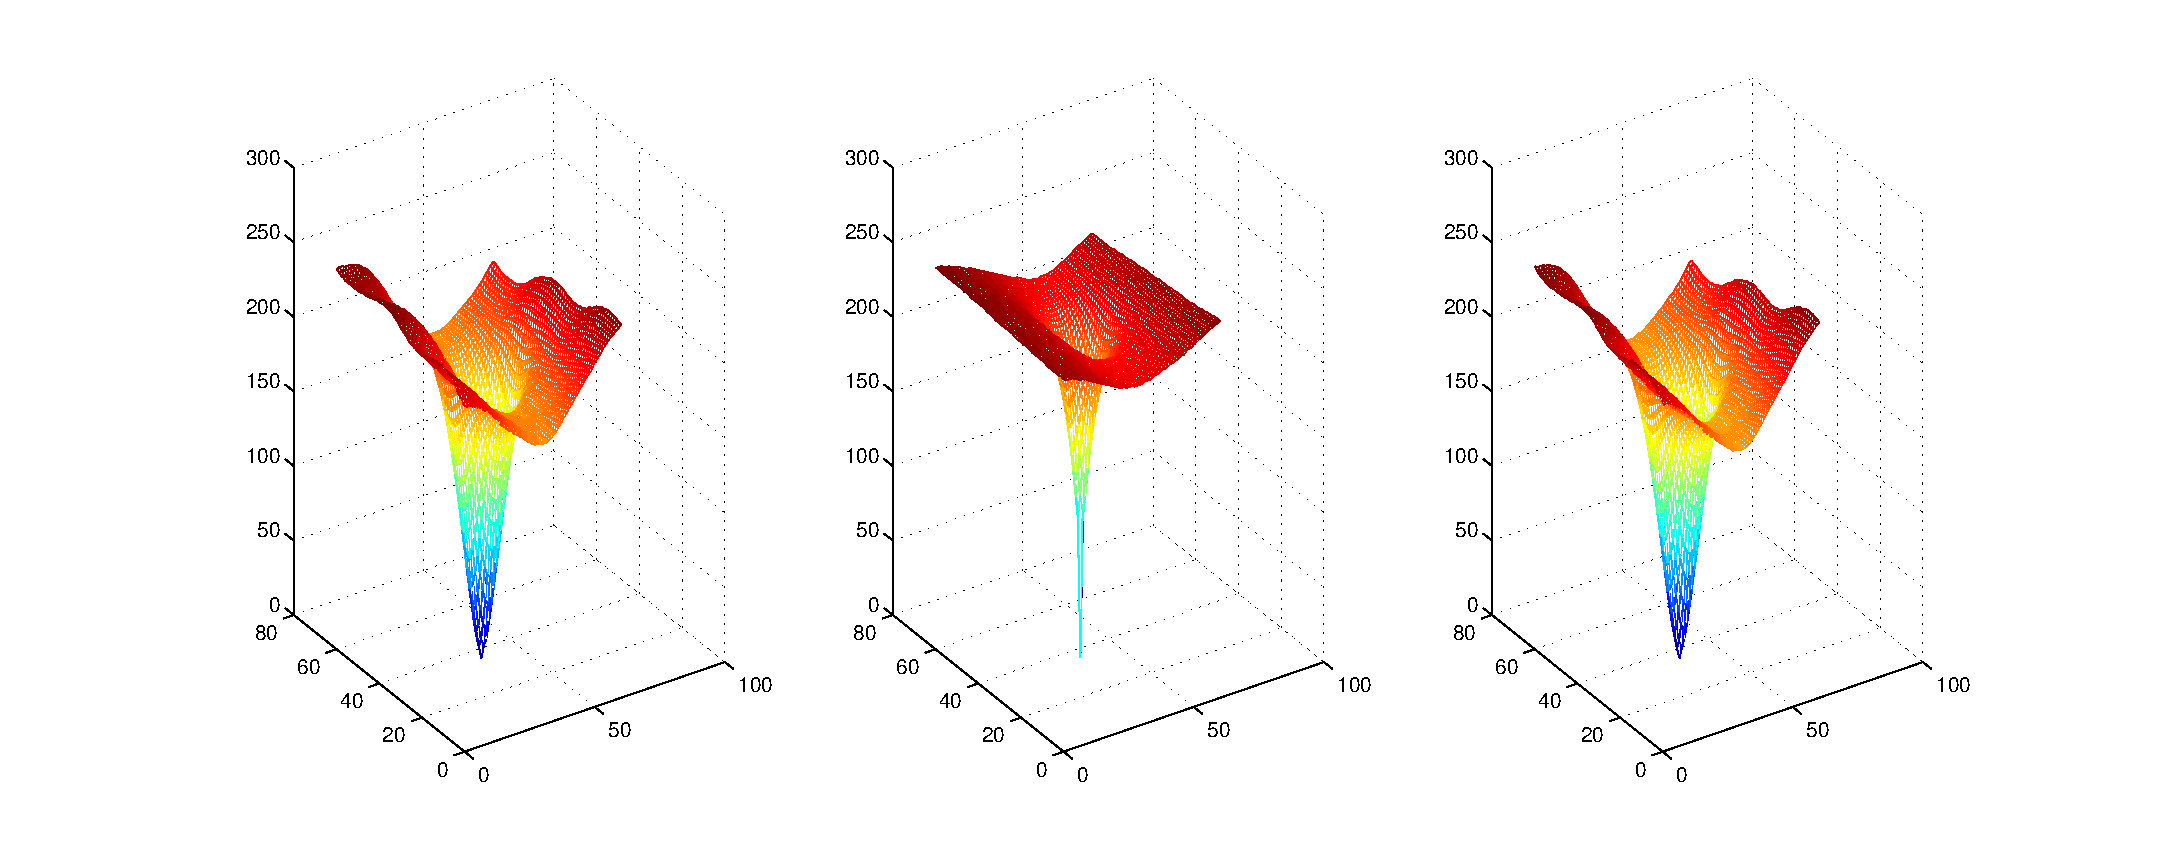
\includegraphics[width=0.95\textwidth]{pictures/Recal3DmetricsCMSArtificial}
\end{center}
\caption{Critères de différence pour une simulation de déplacement}{Valeur du critère de différence pour une simulation de déplacement du spécimen de 5 pixels en x et 5 pixels en y.\\
De gauche à droite :\\
critère de \href{http://www.itk.org/Doxygen/html/classitk_1_1NormalizedCorrelationImageToImageMetric.html}{corrélation normalisé};\\
critère d'information mutuelle de \href{http://www.itk.org/Doxygen/html/classitk_1_1MattesMutualInformationImageToImageMetric.html}{Mattes};\\
critère des \href{http://www.itk.org/Doxygen/html/classitk_1_1MeanSquaresImageToImageMetric.html}{moindres carrés}. }
\label{fig:RecalMetricSynthe}
\end{figure}


La figure~\ref{fig:RecalMetricSynthe} montre que le critère d'information mutuelle de Mattes semble être très précis : il présente un relief presque plat avec un pic correspondant à la translation synthétisée. Cependant, pour cette même raison, ce critère ne peut facilement recaler des images très différentes.
Le critère des moindres carrés, et le critère de corrélation normalisé donnent des résultats à peu près similaires. Il est important de noter que le critère des moindres carrés prend plus de temps à calculer, car il est évalué sur toute l'image (contrairement au critère d'information mutuelle de Mattes qui n'est évalué qu'en 25\% des points sélectionnés aléatoirement, afin de créer un histogramme à 40 catégories).


\begin{figure}[h]
\begin{center}
\leavevmode
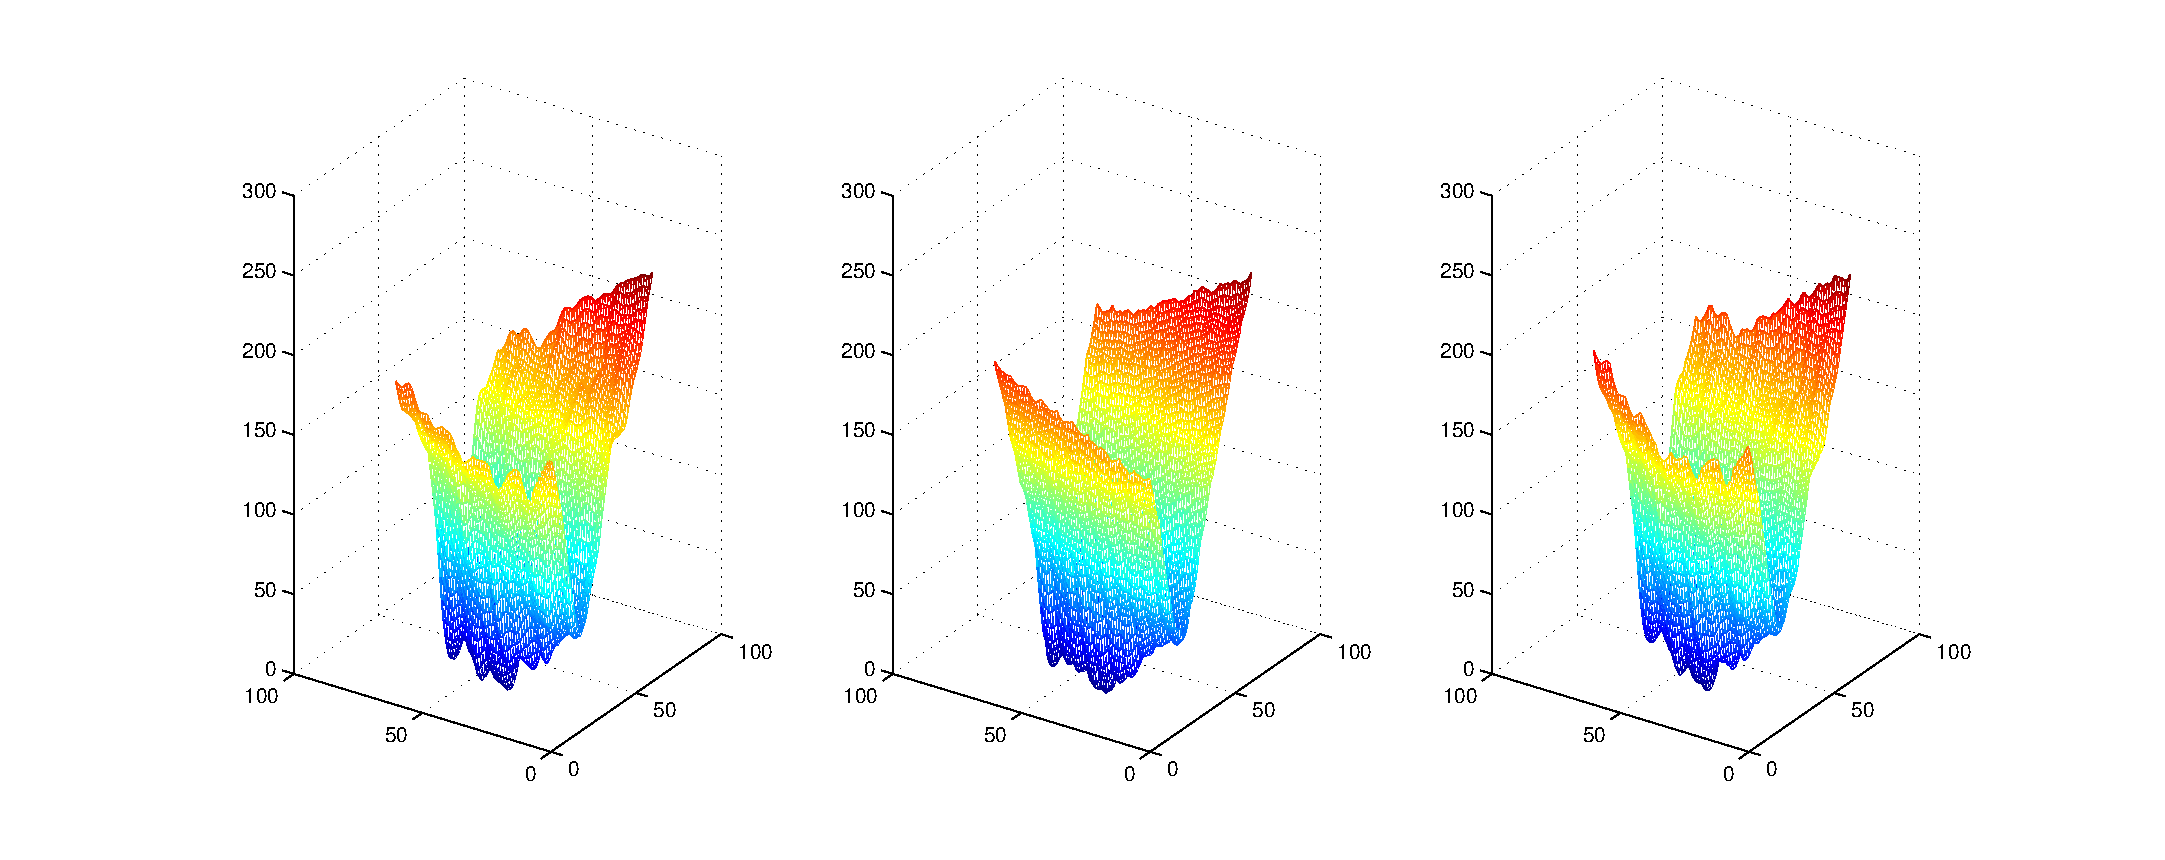
\includegraphics[width=0.95\textwidth]{pictures/Recal3DmetricsCMSReal}
\end{center}
\caption{Critères de différence pour une simulation de déplacement}{Valeur du critère de différence pour un déplacement réel entre deux images acquises à des instants différents.\\
De gauche à droite :\\
critère de \href{http://www.itk.org/Doxygen/html/classitk_1_1NormalizedCorrelationImageToImageMetric.html}{corrélation normalisé};\\
critère d'information mutuelle de \href{http://www.itk.org/Doxygen/html/classitk_1_1MattesMutualInformationImageToImageMetric.html}{Mattes};\\
critère des \href{http://www.itk.org/Doxygen/html/classitk_1_1MeanSquaresImageToImageMetric.html}{moindres carrés}. }
\label{fig:RecalMetricReal}
\end{figure}


La figure~\ref{fig:RecalMetricReal} montre que finalement, sur un essai réel, les trois critères présentent plusieurs minima locaux.
Nous utilisons pour l'instant le critère des moindres carrés pour sa simplicité théorique, mais nous envisageons d'utiliser d'autres critères si les expériences le mettent à défaut.


\subsubsection{Stabilisation de l'acquisition}

La stabilisation de l'acquisition est basée sur les mouvements précédents du spécimen :
nous corrigeons simplement la dernière translation. Le microscope a donc un échantillon de retard.

Afin de pouvoir intégrer la stabilisation au microscope, il a fallu programmer une extension du programme Megacapure.
Megacapture est un programme spécialement développé pour capturer et stocker
des vidéos tri-dimensionnelles de spécimens vivants.
Il a donc fallu intégrer la nouvelle fonctionnalité à Megacapture. Le programme de recalage a été codé en {\C++},
or Megacapture est une macro Visual Basic. Nous avons donc dû créer une interface.
J'ai travaillé avec Paul Cowgill pour créer une interface générique afin de connecter
Megacapture avec des programmes extérieurs. Cela permettant de respecter FC1 du diagramme pieuvre
(figure~\ref{fig:PIEUVRERecal}).

\subsection{Résultats et travail futur}

Afin d'expérimenter les techniques de recalage avec ITK, plusieurs programmes ont été crées, afin de pouvoir évaluer les métriques, et vérifier les temps de calcul. Ces programmes seront aussi utiles à Kishore Mosaliganti, qui travaille sur un projet impliquant du recalage d'images.

Enfin, une interface en Visual Basic, associée à un programme en \C++ a été créée. L'interaction entre les deux applications fonctionne, il ne reste plus qu'à Paul Cowgill d'implémenter le snippet Visual Basic dans Megacapture.

Les figures~\ref{fig:CheckBoardRecalSimu}~et~\ref{fig:CheckBoardRecalReal}  donnent les résultats du programme de recalage, sur un déplacement simulé d'un spécimen statique, puis sur une séquence réelle (le spécimen change de forme).
Le programme met en moyenne une minute trente secondes pour donner un résultat.
Une minute est consacrée à la réduction de l'image, tandis que le recalage prend à peu près trente secondes.
Ces test ont été effectués sur une machine équipée d'un processeur intel "Core 2 Duo" cadencé à 2.53 GHz, et de 4GB de mémoire RAM DDR3. Le programme a été configuré pour être mono-thread\footnote{un programme mono-thread (mono-tâche), s'exécute séquentiellement sur un seul processeur, et n'utilise pas les capacités de calculs parallèles des nouveaux processeurs. Les programmes multi-thread sont souvent bien plus rapides que les programmes mono-thread, cependant, la non linéarité dans l'exécution entraine des difficultés lors du débuguage.}. Le "mutithreading" est déjà implémenté, mais pour les tests, nous préférons rester sur une architecture simple à débuguer.


\begin{figure}[h]
  \centering
  \subfloat[Image du poisson zèbre fixe. La même image translatée d'une distance correspondant  rayon moyen du noyau d'une cellule, selon les deux dimensions de l'espace est utilisée comme image mobile.]{\label{fig:RecalFixBefore}\includegraphics[width=0.5\textwidth]{pictures/RecalSimuFix}}\\
  \subfloat[Damier des images avant recalage.]{\label{fig:RecalSimuCheckBefore}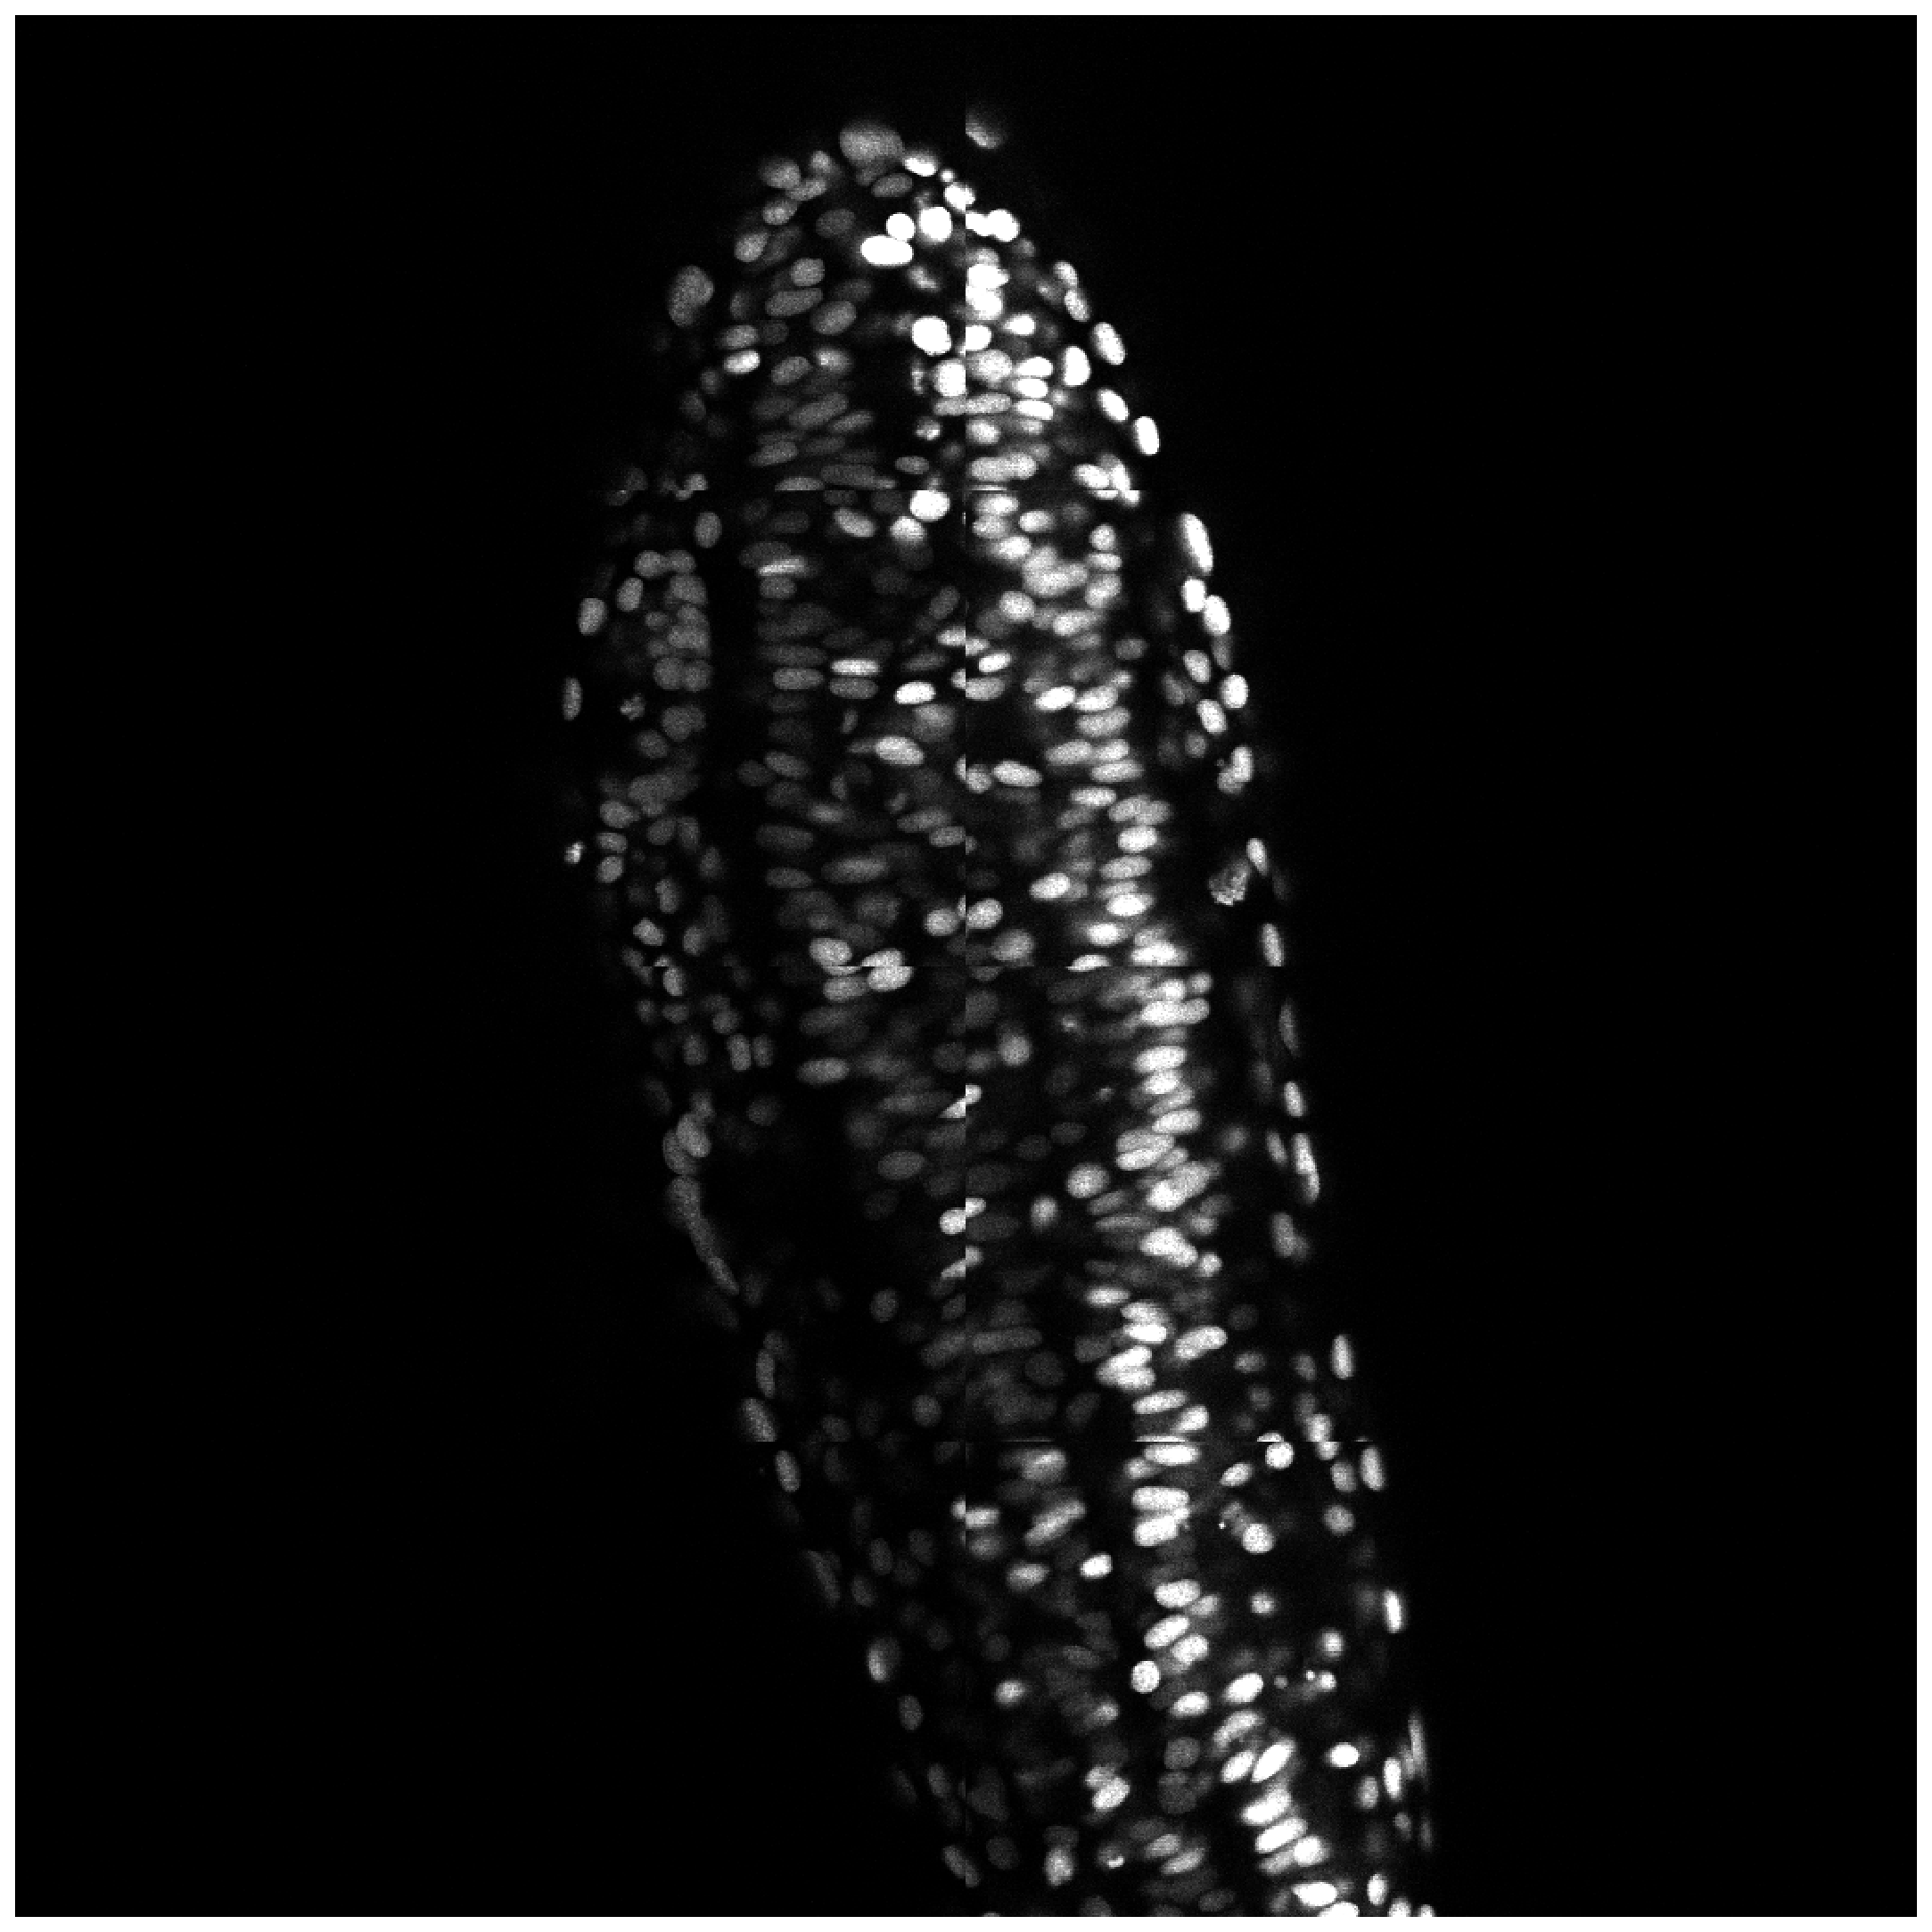
\includegraphics[width=0.5\textwidth]{pictures/RecalCheckBeforeSimu}}                
  \subfloat[Damier des images après recalage; Nous n'apercevons plus le damage, le recalage est donc précis.]{\label{fig:RecalSimuCheckAfter}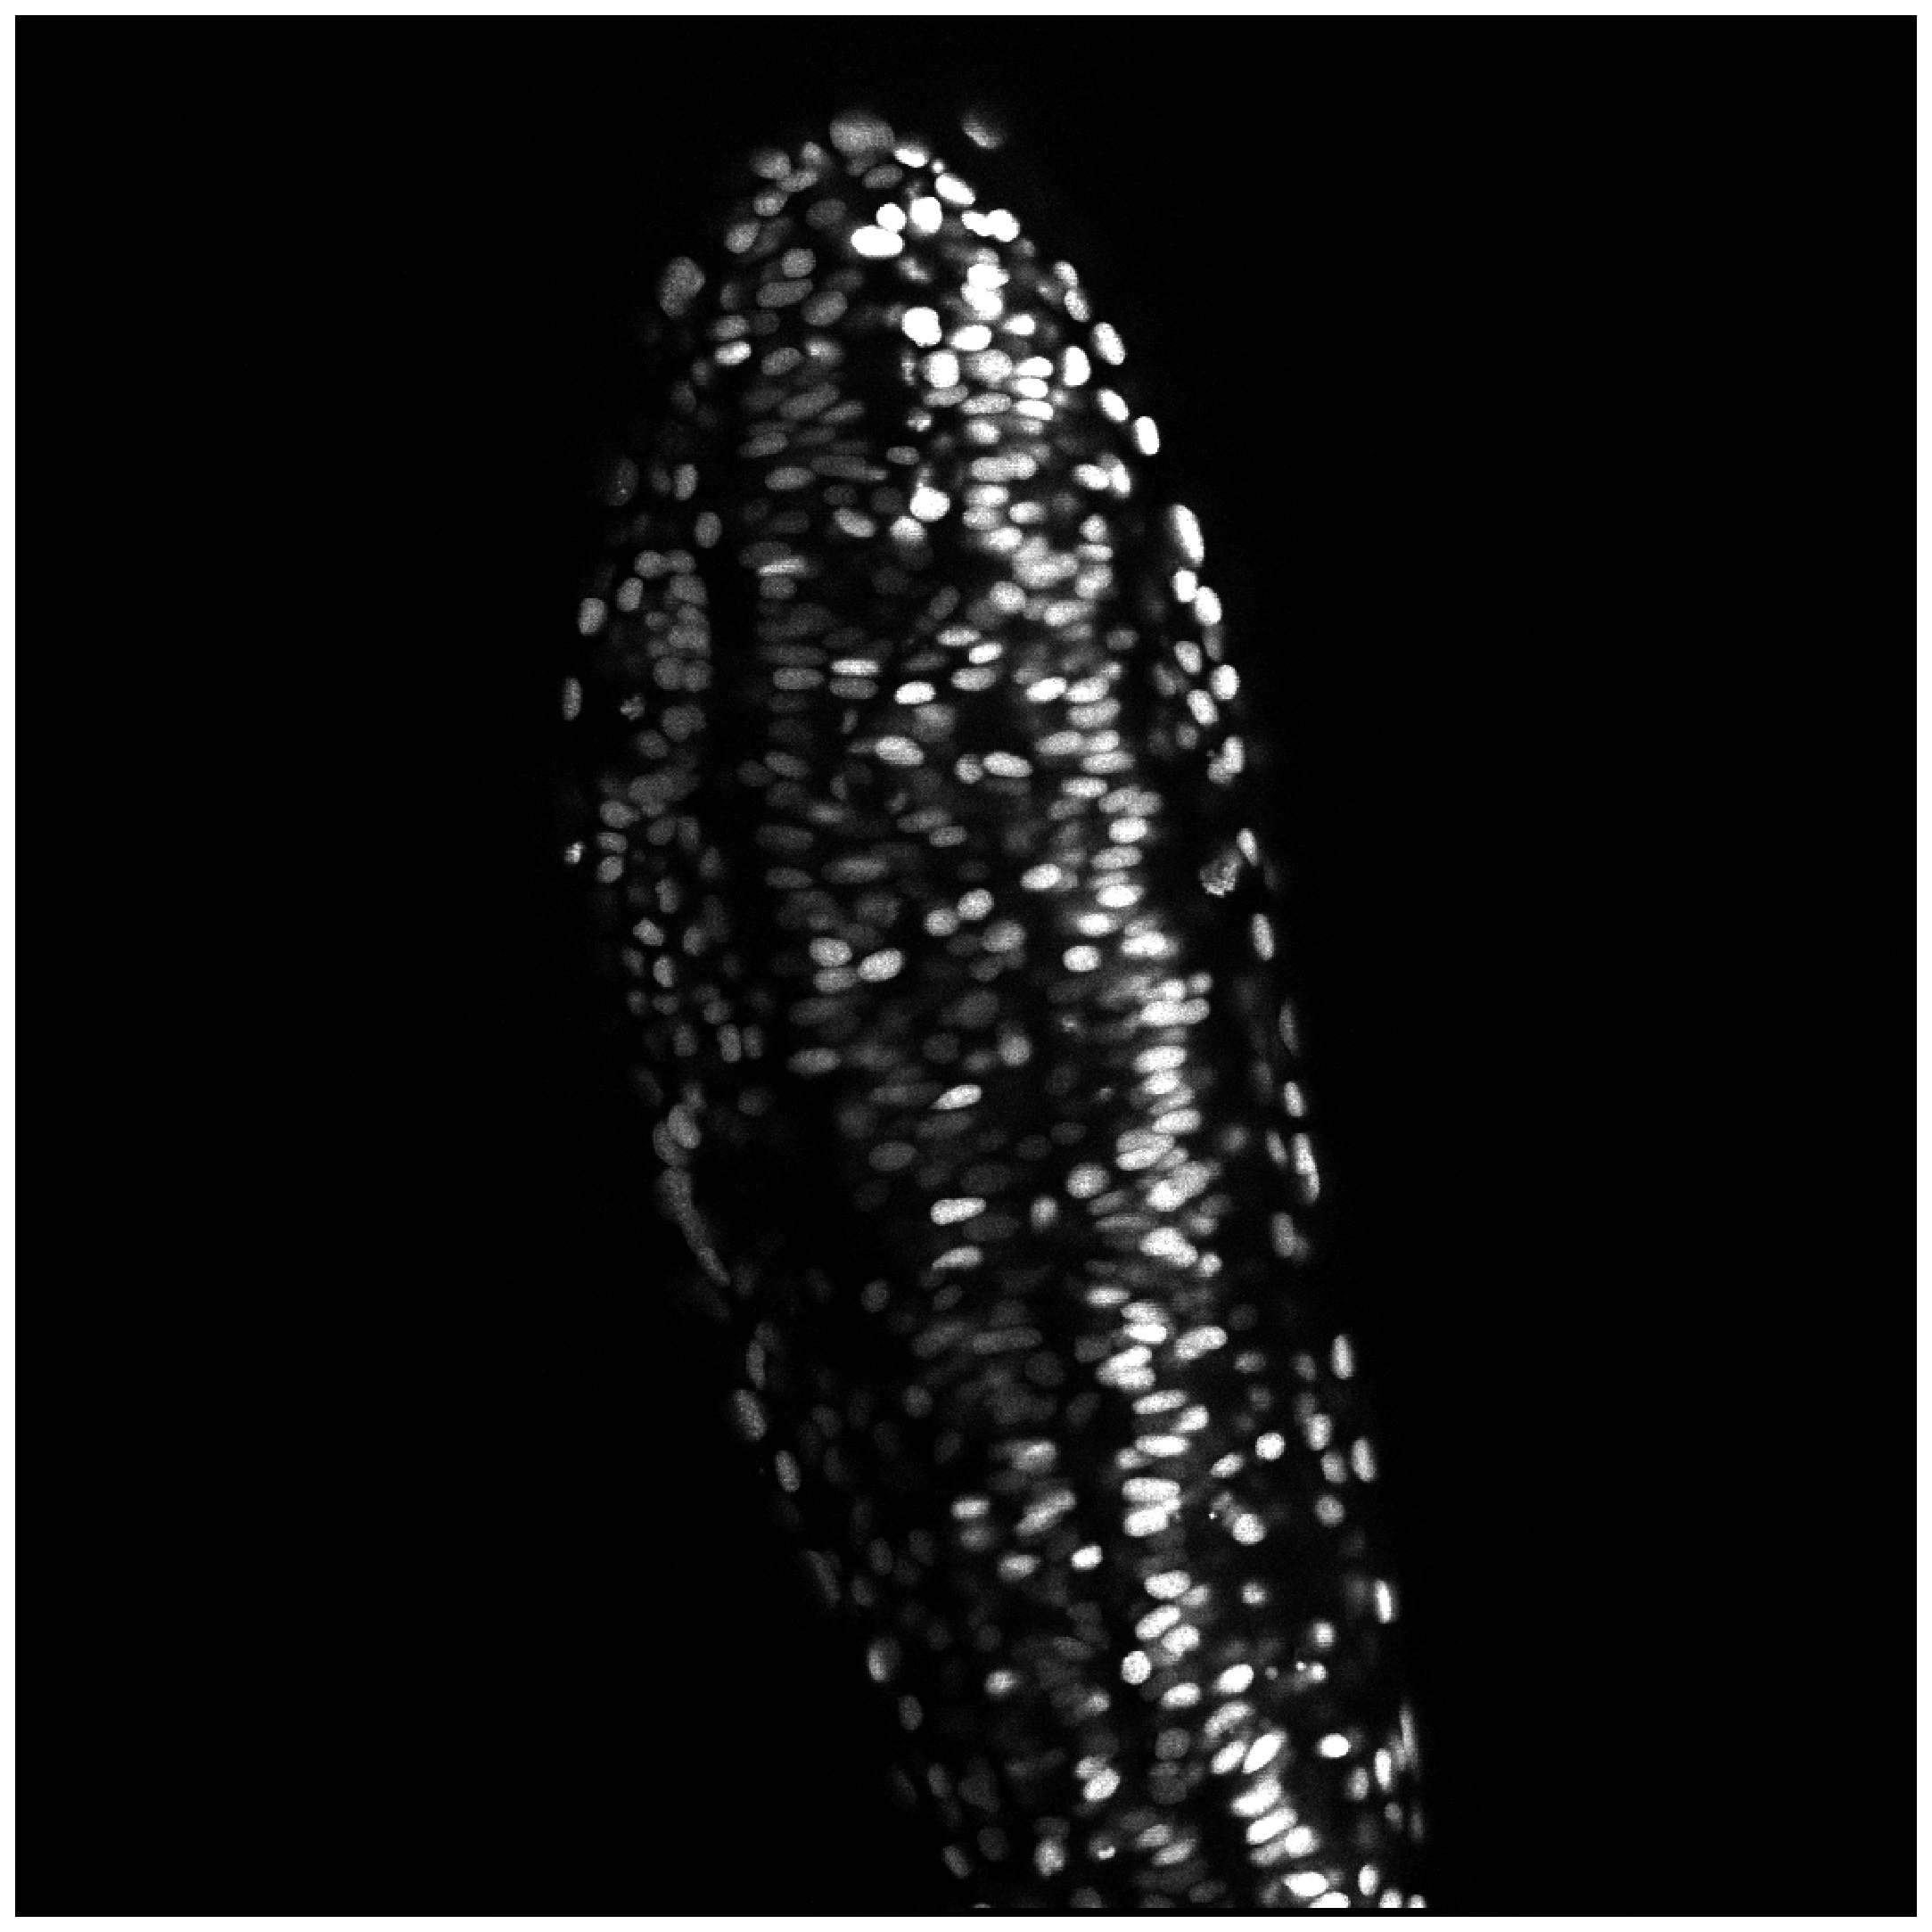
\includegraphics[width=0.5\textwidth]{pictures/RecalCheckAfterSimu}}
  \caption{Programme de recalage une image du poisson zèbre translatée artificiellement.}
  \label{fig:CheckBoardRecalSimu}
\end{figure}



\begin{figure}[h]
  \centering
  \subfloat[Image du poisson zèbre à t=0.]{\label{fig:RecalRealFix}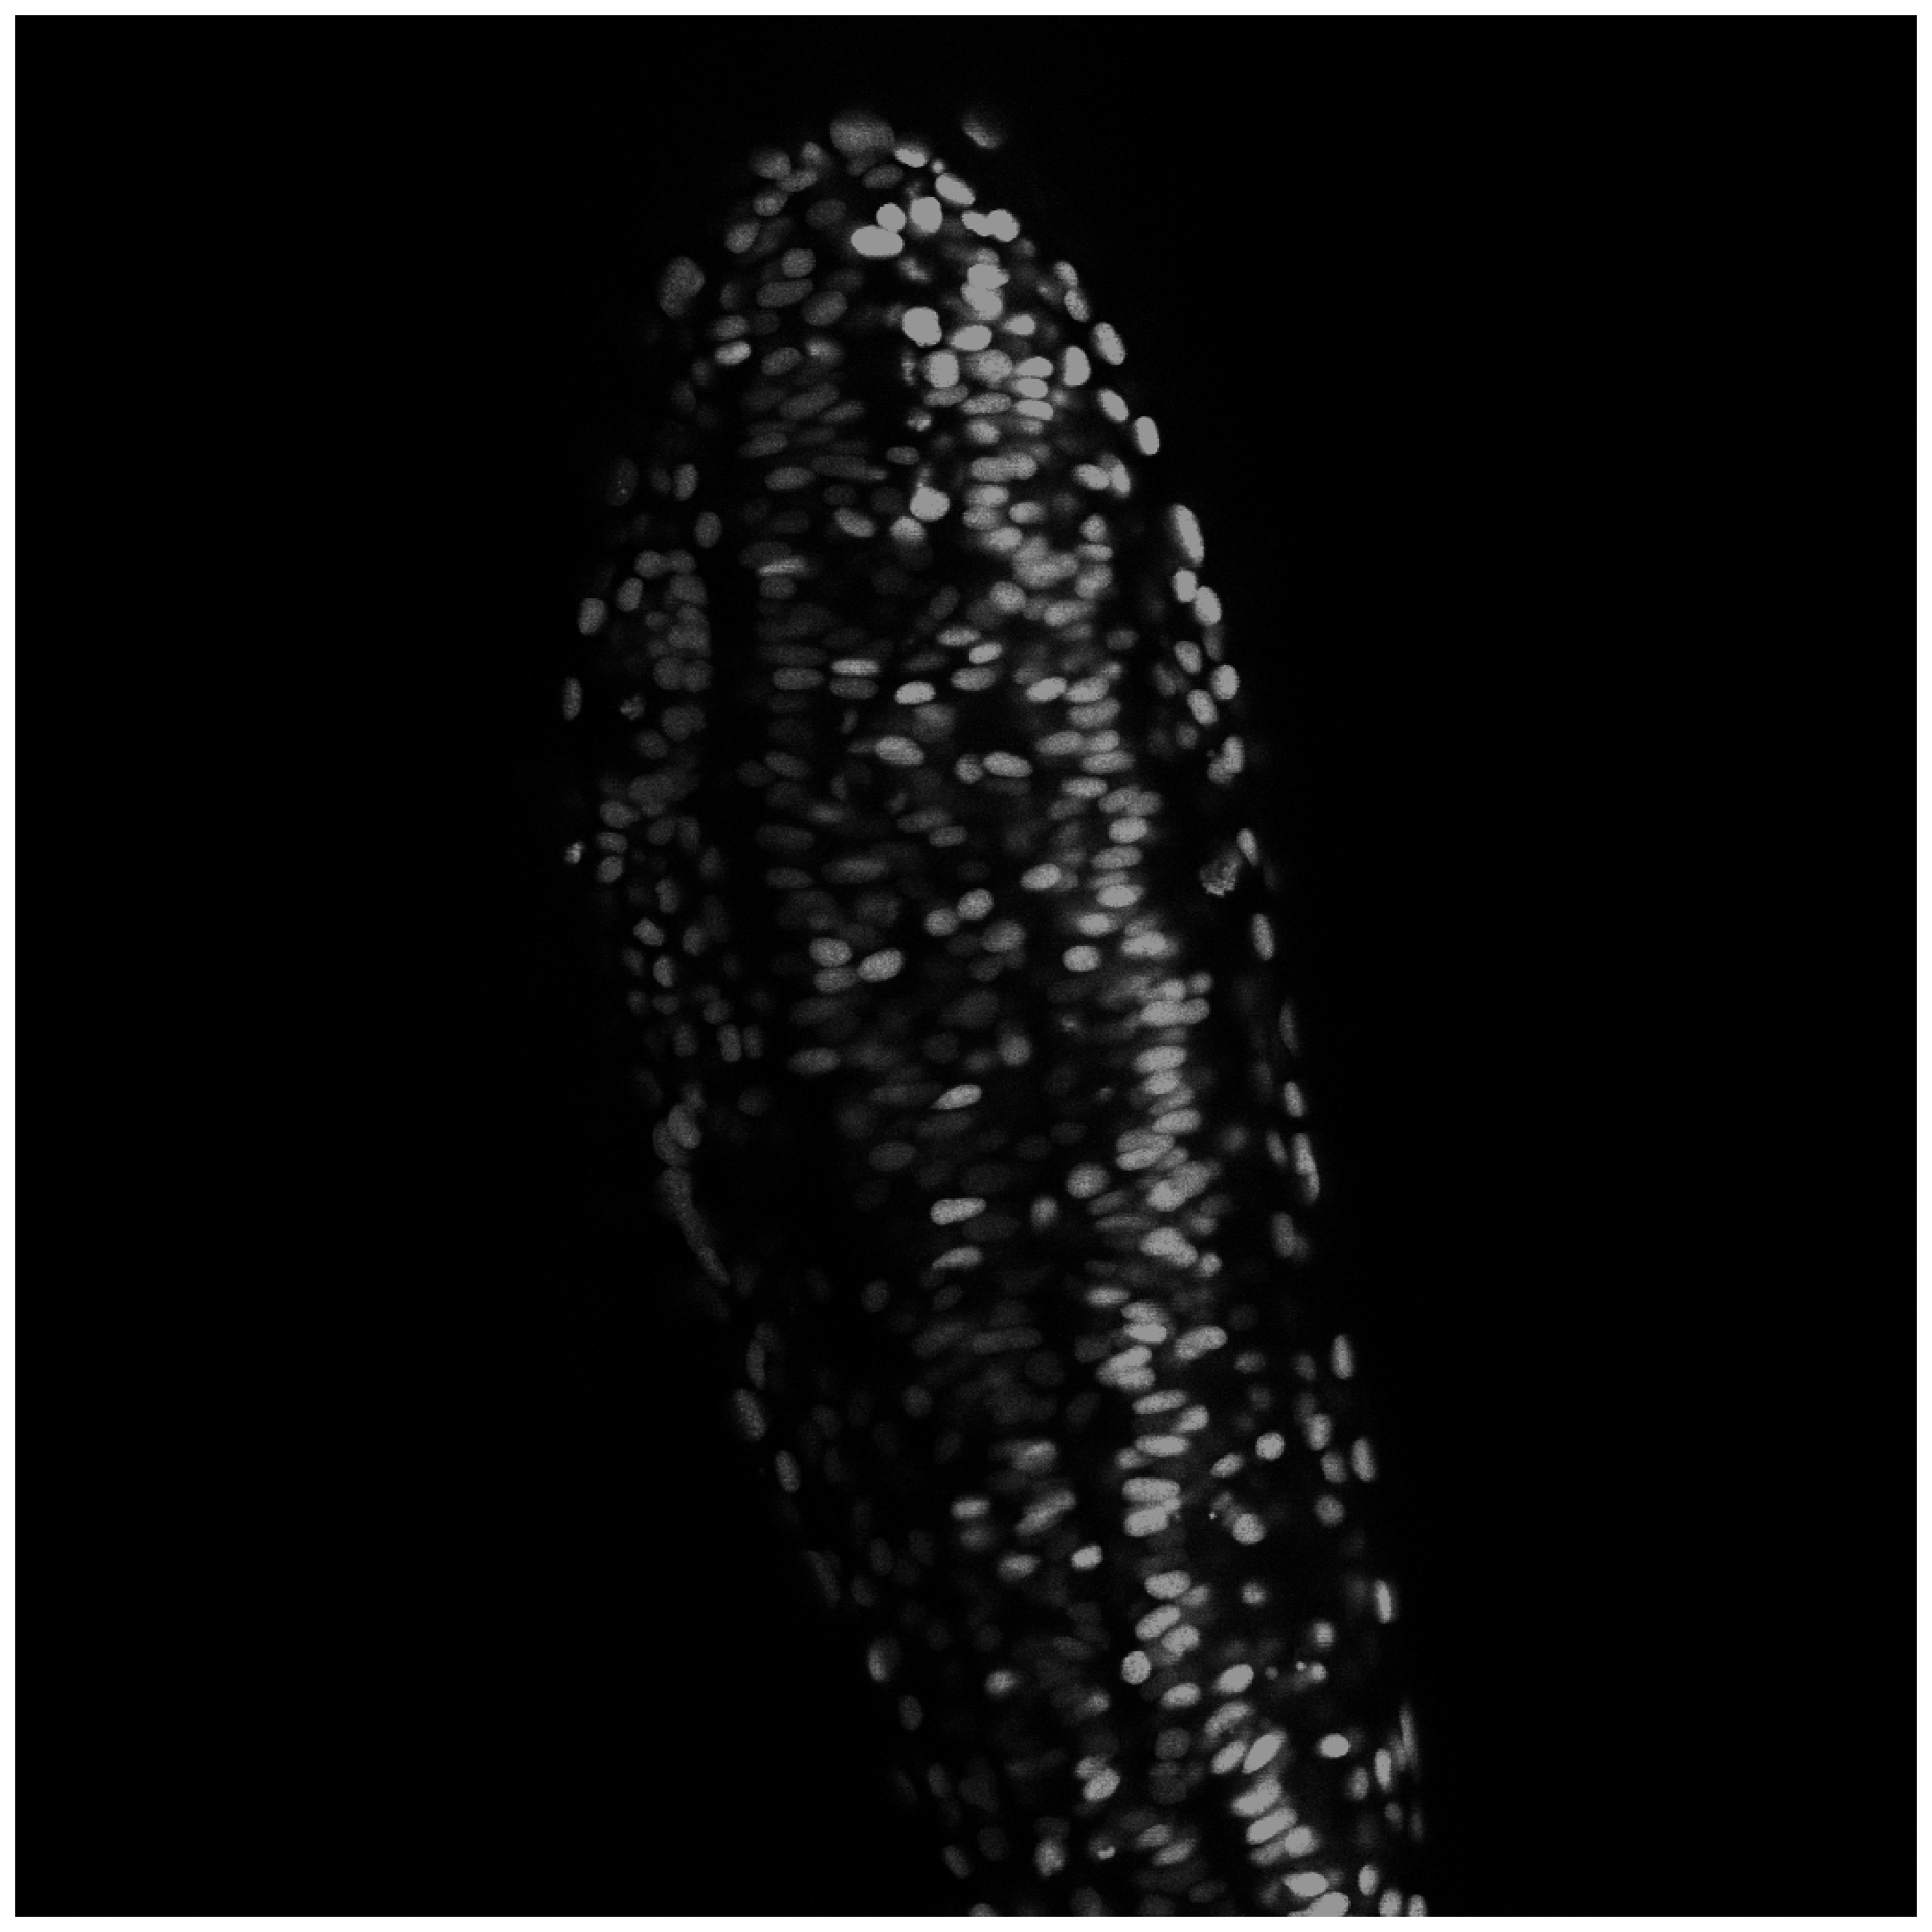
\includegraphics[width=0.5\textwidth]{pictures/RecalRealFix}}
  \subfloat[Image du poisson zèbre à t=2minutes.]{\label{fig:RecalRealMobil}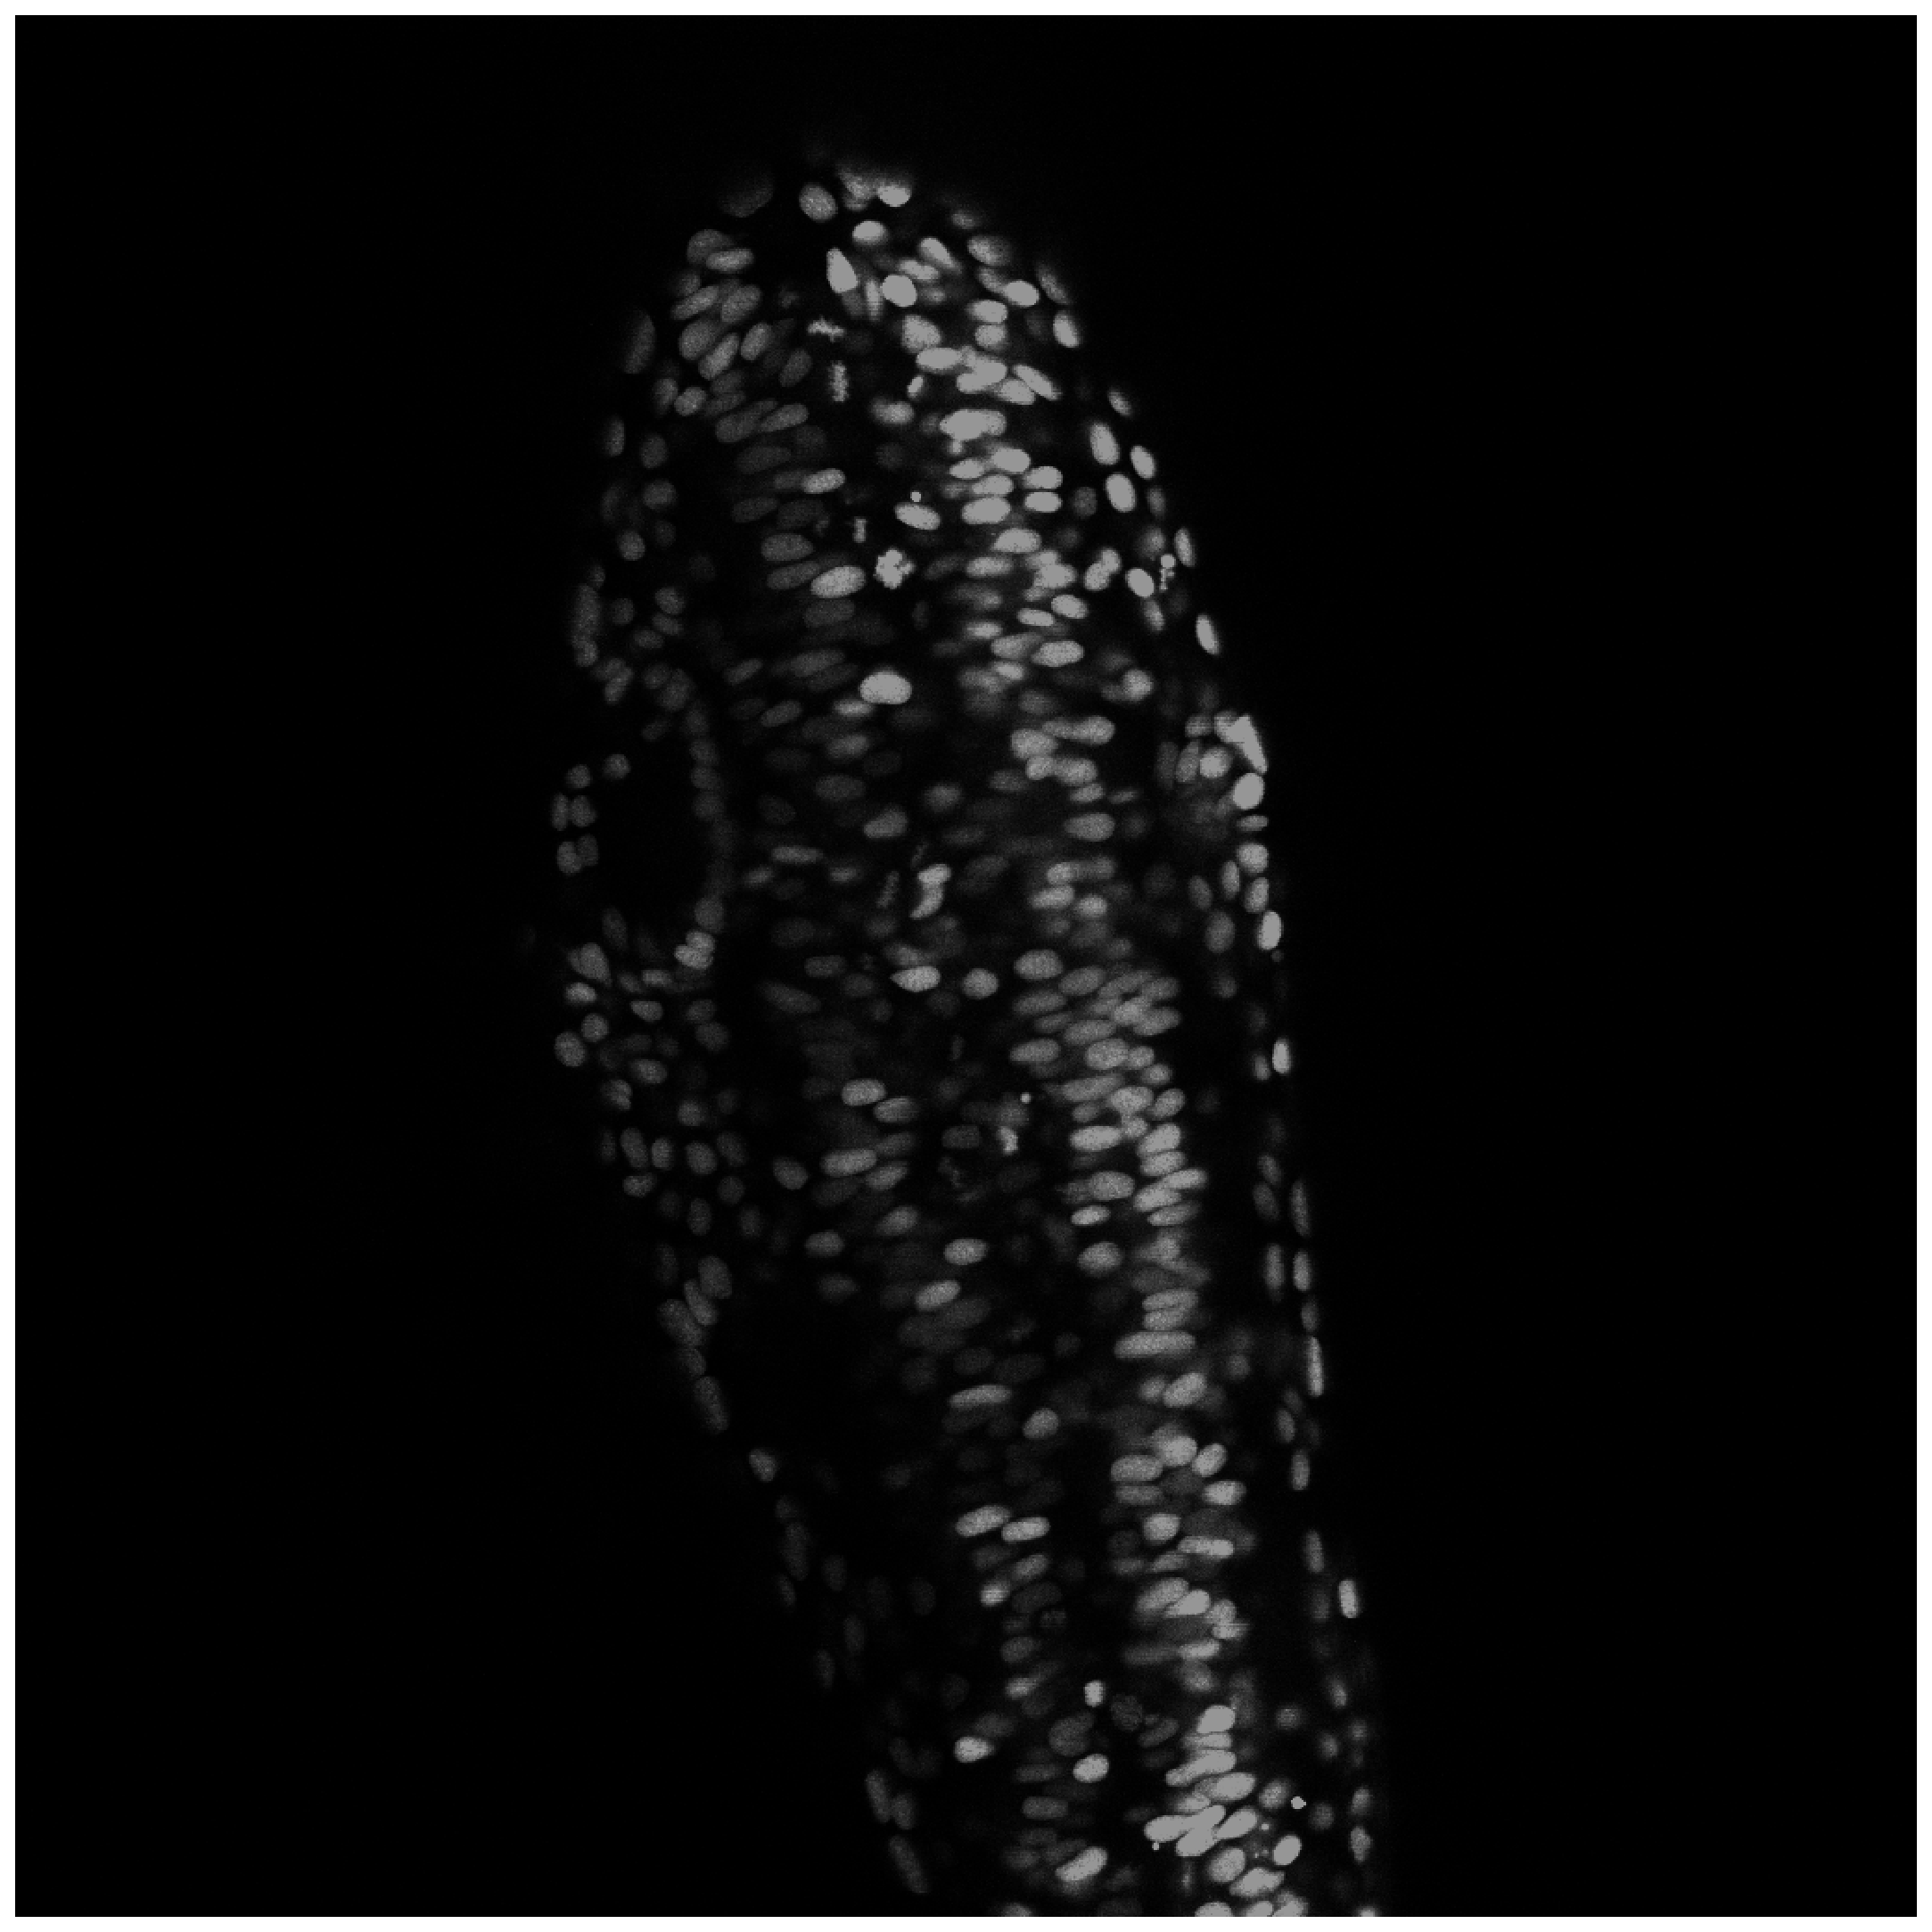
\includegraphics[width=0.5\textwidth]{pictures/RecalRealMobil}}\\
  \subfloat[Damier des images avant recalage; des lignes rouges ont été tracées pour attirer l'attention vers les zones mal alignées.]{\label{fig:RecalRealCheckBefore}\includegraphics[width=0.5\textwidth]{pictures/RecalCheckBeforeReal}}                
  \subfloat[Damier des images après recalage; des lignes rouges ont été tracées pour attirer l'attention vers les zones bien alignées après le recalage.]{\label{fig:RecalRealCheckAfter}\includegraphics[width=0.5\textwidth]{pictures/RecalCheckAfterReal}}
  \caption{Programme de recalage sur une vidéo réelle du poisson zèbre durant son développement}
  \label{fig:CheckBoardRecalReal}
\end{figure}


L'analyse de la figure~\ref{fig:CheckBoardRecalSimu} montre que le recalage s'effectue correctement sur un déplacement simulé. Le damier de vérification
\footnote{Les damiers de vérification sont souvent utilisés en recalage, afin de visualiser le résultat d'une technique de recalage. L'image "fixe" et l'image "mobile" sont représentées dans le même repère. Le damier alterne l'image fixe et l'image mobile, si le damage est clairement visible, les images sont mal alignées. On présente en général un tel damier avant d'utiliser l'algorithme de recalage afin de montrer les mauvais alignements, puis après, en appliquant la transformation estimée par l'algorithme de recalage à l'image mobile.}
montre que l'on obtient deux images identiques après l'exécution de l'algorithme.
Cela prouve que la simplification de l'image (moyennage puis sous-échantillonnage)
n'entraine pas de baisse de précision visible du recalage.

L'analyse de la figure~\ref{fig:CheckBoardRecalReal} montre que le recalage s'effectue correctement,
les caractéristiques importantes des images sont bien mieux alignées après le recalage.
Grâce à la simplification des images, le recalage se focalise sur les caractéristiques importantes des images.





Nous sommes donc encore dans la phase d'intégration et de test sur ce projet.
Il faut maintenant faire des expériences. Nous comptons tout d'abord tester le projet
sur des objets que nous bougerons manuellement, pour vérifier la réponse du Microscope.
Nous voulons ensuite tester notre programme sur un poisson zèbre en développement, au cours d'une session d'imagerie.

Il existe de nombreuses pistes pour étoffer les fonctionnalités de ce projet, en voici quelques unes :\begin{itemize}
  \item Nous envisageons dans le futur d'utiliser un filtre de Kalman afin d'estimer
  le déplacement qui aura lieu à la prochaine acquisition, en connaissant les déplacements passés. Ce filtre particulier incorpore un modèle évolutif du système et peut donc corriger(filtrer) les mesures précédentes pour estimer au mieux la 
  \item Plutôt que d'utiliser un recalage rigide, il pourrait être judicieux d'utiliser un recalage "souple",
  qui donne un champ de déformation (déplacement de chaque point).
  Ainsi, le chercheur pourra sélectionner une zone d'intérêt sur un spécimen,
  et le programme, à partir du champ de déplacement dans cette région, pourra calculer
  le déplacement moyen de l'organe visé.
  \item Le temps d'exécution peut être raccourci en modifiant le programme pour qu'il soit multi-tâches.
  Nous pouvons aussi améliorer la qualité du recalage en utilisant un débruitage et une réduction de la résolution
  des images à recaler, par ondelettes
  Cela nous permettrait d'obtenir une meilleure image grossière sur laquelle baser l'algorithme.
  \item Nous pouvons enfin utiliser un recalage "pyramidal" qui permet d'estimer tout d'abord un déplacement
  grossier (sur des images faible résolution), pour ensuite donner un recalage plus précis (sur des images haute résolution).
\end{itemize}




\clearpage




%% Chapitre sur le rapport de recherche :


\chapter{Rapport de recherche} 

\section*{Introduction}

\subsection*{}
Je présente deux dans cette partie, la démarche recherche que j'ai eue pendant le PFE. Il s'agit tout d'abord de bien prendre connaissance du sujet. Cette prise de connaissance permet de voir quels problèmes persistent. Il faut ensuite trouver une solution à ces problèmes, afin de pouvoir avancer dans sa résolution.

La difficulté en recherche, est que bien souvent, il n'existe pas de solution dans le domaine étudié.
Il faut donc passer par une phase de bibliographie, pour étudier l'état de l'art,
et éventuellement apprendre de nouvelles théories.
Le domaine du traitement de l'image est une science particulière car beaucoup d'algorithmes sont inventés,
mais très peu sont diffusés ou applicable a divers types d'images.
Il faut donc reprogrammer les algorithmes présentés dans les publications scientifiques et vérifier leur performance.
Il faut enfin trouver des idées innovantes pour résoudre les problèmes posés, et expérimenter.

\subsection*{}
J'ai travaillé, pendant mon PFE au Megason Lab sur la segmentation d'images obtenues par microscopie fluorescente.
Les données sont quadri-dimensionnelles (espace et temps), et représentent des régions du poisson zèbre (oreille, colonne vertébrale...). Il s'agit de vidéos prises pendant le développement du spécimen. Nous pouvons bien discerner les différentes cellules du poisson, ainsi que leur noyaux. Ces éléments sont donc la base du modèle que nous tentons de créer. Il faut donc être en mesure de détecter et suivre ces cellules au cours du temps. Le modèle devra aussi intégrer les informations morphologiques de chaque cellule.

Ce modèle fait l'objet d'une proposition de thèse : Modèle numérique cellulaire de poisson zèbre ( cells lineage registration in microscopy) durant laquelle j'aimerais poursuivre mes travaux.

Avant d'arriver au Laboratoire, j'ai travaillé sur la membrane cellulaire. J'ai ensuite concentré mes recherches sur la détection et la localisation de noyaux.

\section{Segmentation de la paroi cellulaire par ensembles de niveaux}

Le but initial du PFE etait la segmentation de la paroi cellulaire. il s'agit d'une fine membrane séparant les multiples cellules. Elle s'étend sur tout le spécimen a analyser. Il s'agit donc d'un volume important et complexe.

\subsection{Étude du problème}

J'ai tout d'abord cherché à comprendre le problème posé : sur quelles données allaient se baser la détection, existe-t'il des solutions pour segmenter ce genre de données.

\subsubsection{Les données}
Les images sont acquises a travers un système optique. L'excitation par un laser entraine la fluorescence de certaines parties de la cellule, marquées par une molécule émettant de la lumière dans un spectre dépendant du marqueur utilisé.

Le système a donc une réponse impulsionelle bien visible dans les données. Un point correspond grossièrement a une gaussienne étalée dans les trois dimensions de l'espace, et plus particulièrement selon l'axe perpendiculaire au plan de focalisation.

Il existe aussi un bruit du au dispositif électronique d'acquisition. De plus, la fluorescence n'étant pas repartie de manière homogène, il existe des "trous" et de la saturation dans les données.
\TODO{inserer des images illustrant les problemes}


J'ai choisi de me focaliser sur trois difficultés afin de trouver des solutions :
\begin{description}
  \item [problème du bruit] : quel filtrage appliquer aux images, afin de les débruiter.
  \item [problème de l'absence de données] : comment introduire des à priori de forme de la membrane
  pour palier à l'absence d'information ?
  \item [problème de la non homogénéité des intensités]  : comment segmenter un objet
  qui n'occupe pas les mêmes intensités selon sa position dans l'espace.
\end{description}


\subsection{Utilisation de la théorie des ensembles de niveaux}

L'outil choisi pour segmenter la paroi cellulaire, est base sur les ensembles de niveaux (levels-sets). Cette théorie consiste en l'évolution d'un front. Cette évolution est représentée par une fonction implicite qui évolue itérativement. Le front (bords de la zone segmentée) est souvent représenté par le niveau zéro de cette fonction implicite.
Les Level sets, au travers de leur critère d'évolution, permettent d'avoir une grande flexibilité quand aux mesures a considerer lors de l'evolution du front. Cette évolution est représentée par un critère d'énergie, le problème de segmentation par level set est donc un problème d'optimisation.

\subsection{des idees}



Afin d'éliminer le bruit sans détériorer la membrane, le principe de l'érosion dilatation a été mis en oeuvre. Il s'agit d'une methode rapide qui donne de bons resultats


idee de la mediane
idee morphologie
idee localisation
\subsection{resultats}
idee mediane
idee morphologie
idee localisation
\subsection{travail futur}
rapidite



\section{Detection et localisation des cellules}

Nous basons nos méthodes de segmentation sur une initialisation au centre des cellules. Nous avons donc besoin de détecter un maximum de cellules afin de trouver un point a l'intérieur de ces dernières. Des methodes ont ete proposees, cependant, chacune est adaptee a un type d'image particulier.
Cels algorithmes de détection sont aussi souvent appelles algorithmes de "seeding" car ils permettent d'obtenir des points a partir desquels une segmentation peut etre initialisee, afin de delimiter les bordures des noyaux, ou les membranes cellulaires.

\subsection{demarche}

Nous avons developpe une methode combinant l'information provenant des noyaux et de la membrane des cellules. Cette methode doit etre evaluee, donc comparee a d'autres methodes existantes. Ce processus d'evaluation nous permettra aussi de trouver les points forts et les points faibles des algorithmes. Nous pourrons ainsi eventuellement utiliser des techniques de fusion d'information pour combiner les resultats de differents algorithmes.
La creation d'un "framework" d'evaluation passe donc par plusieurs etapes : l'implementation des algorithmes existants, afin de les tester sur des images synthetiques puis reelles, la creation de criteres d'evaluation appropories, et l'observation des resultats. Nous avons aussi initié un travail afin de proposer une nouvelle methode de detection de cellules basee sur la decomposition en ondelettes.


\subsection {description des algorithmes evalues}



\subsubsection{chaine de traitement de l'image}

partie commune
Nous nous focalisons sur une classe d'algorithmes traitant l'information issue de l'image des noyaux cellulaires, apres une detection des zones d'interet (binarisation de l'image). Ces algorithmes fonctionnent aussi souvent avec une extraction de maxima locaux en dernier traitement.
Nous choisissons d'utiliser la même binarisation, et la meme methode d'extraction de maximas locaux pour les deux algorithmes afin de focaliser l'etude sur la technique de detection des centres des noyaux.

\subsubsection{description des algorithmes}
\paragraph{le Laplacien de la Gaussienne ameliore}
Nous avons decide d'implementer l'algorithme presente dans \cite{al2009improved}. La methode utilisee est celle du Laplacien de la Gaussienne (LoG). Une methode eprouveee qui s'est montree tres robuste dans d'autres applications telles la detection de points de reperes pour le recallage photographique.



\paragraph{Kishore}

\TODO{Ask Kishore more infos}


\subsection {evaluation}
%\begin{tabular}{|c|c|c|c|c|}
%\hline  & Matching & UnMatching & Missed & Accuracy \\ 
%\hline A1 & 10 & 3 & 1 & 71% \\ 
%\hline A2 & 9 & 2 & 3 & 64% \\ 
%\hline 
%\end{tabular} 



\subsection {conclusion}


\subsection {proposition}



\subsection {planning}


\subsection{resultats}

\subsection{proposition}









\chapter{Conclusion du PFE}


\section{Conclusion de la partie ingénierie}

Durant ce PFE, j'ai travaillé sur des projets très variés.
Ces projets étaient motivés par des objectifs scientifiques et nécessitaient chacun un haut niveau de technicité.

J'ai eu l'occasion d'apprendre énormément,
notamment dans le domaine des sciences informatiques,
et du traitement de l'image.

J'ai aussi découvert le milieu de la recherche, dont l'organisation est
totalement différente de celle du milieu industriel.
La hiérarchie, et les intérêts de chaque scientifique sont moins apparents que dans une entreprise et ce PFE a été riche en enseignements sur ce plan.
Je suis parvenu à très bien m'intégrer dans l'équipe du Megason Lab en général,
et à établir de bonnes relations de travail avec les divers scientifiques
impliqués dans les projets sur lesquels j'ai travaillé.

Cela m'a permis d'acquérir une base solide pour mener des recherches dans ce domaine.
Après une importante phase d'apprentissage, je maitrise maintenant des librairies de renom
(ITK, VTK,Qt), les systèmes unix, et la gestion de versions.

J'ai pu aussi établir des contacts dans la communauté
des traiteurs d'image par le biais de collaborations
(Matthiew MacCormick), ou de d'"ateliers" (workshops) internationaux
(participation à la NAMIC
\footnote{La National Alliance for Medical Image Computing (NAMIC), est un réseau de professionnels de traitement d'images médicales. Ce réseau organise des conférences et des ateliers de travail ("workshop"), durant lesquels les scientifiques peuvent collaborer.}
summer project week, au Massachusetts Institute of Technologies).


\section{Projet professionnel}

Ce PFE s'inscrit dans un projet professionnel construit durant ma scolarité à l'INSA de Lyon.
Mon inscription à l'INSA de Lyon a été grandement motivée par l'ouverture de l'école à l'international. J'ai ainsi effectue mon stage ouvrier en Afrique du Sud. Profitant d'une première expérience professionnelle à l'international.

Lors de ma seconde année a l'INSA de Lyon, j'ai choisi l'option SCiences et ANglais (SCAN).
Cette filière regroupe les élèves ayant un niveau suffisant pour pouvoir suivre la formation généraliste en anglais.
Elle s'accompagne d'une bourse pour un bref séjour linguistique dans une université étrangère.
J'ai profité de ce financement pour aller au Trinity College en Irlande où
j'ai pu avoir ma première expérience académique à l'étranger.

J'ai ensuite choisi le département
Génie Électrique qui permet de bénéficier d'un grand panel de compétences,
notamment dans des domaines rattachés à l'électronique et l'informatique.


Continuant l'expérience internationale, j'ai effectué mon stage industriel au
Fraunhofer Institute, Center for Manufacturing Innovation, aux États Unis.
J'ai été impliqué dans un projet de grande ampleur, financé par le département de la défense américain.
Ce stage m'a énormément apporté en plus de l'expérience technique : il s'agissait d'une immersion dans la culture américaine, et j'ai eu une première expérience managériale en dirigeant une équipe d'ouvriers.
C'est après ce stage que j'ai passé le test TOEIC validant un très bon niveau d'expression et de compréhension en anglais,
avec un score de neuf cent quatre-vingt sur neuf cent quatre-vingt dix.


Le PFE au Megason Lab possède des attraits indéniables :
il s'agit d'un stage de recherche perfectionnant mes connaissances en traitement de l'image.
Il s'agit aussi d'une expérience internationale dans une université renommée : Harvard Medical School.
Ainsi, en plus de prendre plaisir à travailler en recherche, j'ouvre la porte à de nombreuses opportunités professionnelles.

Comme je suis intéressé par les domaines techniques,
je compte profiter de l'opportunité de poursuivre mes études pour obtenir un doctorat en mathématiques appliquées,
au cours d'une thèse élaborée en collaboration avec le laboratoire CREATIS (INSA Lyon)
et le laboratoire Megason (Harvard Medical School).
Je passerai ainsi la moitié de mon temps en France, et l'autre moitié aux États Unis.
En plus de pouvoir travailler sur un domaine passionnant,
je pourrai ainsi bénéficier d'une équivalence avec un PhD (diplôme très reconnu à l'international). 

Je compte ensuite mettre en valeur ma capacité a travailler dans un contexte international,
dans des domaine à haute technicité pour trouver un emploi  dans le secteur privé.
Je pourrai mettre en avant mes capacités en traitement du signal pour travailler dans le médical ou l'aéronautique.

Mon ambition à long terme est de migrer vers des responsabilités managériales après avoir une très bonne maitrise de la technique.

\chapter*{Remerciements}
\phantomsection
\addcontentsline{toc}{chapter}{Remerciements}

Je tiens à remercier tout particulièrement, pour leur aide et leur participation au PFE, les personnes suivantes :

\begin{center}
Sean MEGASON\\
Kishore MOSALIGANTI\\
Arnaud GELAS\\
Olivier BERNARD\\
Rémy PROST\\
Matthiew MACCORMICK\\
Isabelle BLOCH\\
Nicolas RANNOU\\
Lydie SOUHAIT\\
Amelia GREEN\\
Nikolaus OBHOLZER\\
Ramil NOCHE\\
Raghav K. PADMANABHAN\\
Luis IBANEZ\\
\end{center}


\appendix

%Annexes du rapport d'ingénierie



\chapter{Librairies utilisées pour le projet de Comparaison d'images}


\paragraph{La librairie "Insight ToolKit" (ITK)} est un projet open source initialement destiné au recalage et a la segmentation d'images medicales. ITK a été programmée en \C++ , en utilisant des techniques de codage avancées (templates, modification de la syntaxe standard et ajout de fonctionnalités au langage \C++ par le biais d'idiomes) , ainsi que l'outil de développement cross-platform CMake, et communautaires (SVN, puis GIT). 
Cette librairies est construite sur un système de "Templates", qui lui permet de s'adapter à diverses données. Elle propose une architecture centrées sur un flux de données, traité par différents filtres que l'on connecte ensemble.
Cette collection d'algorithmes ne cesse de s'agrandir grâce à la philosophie open-source. Le spectre des applications d'ITK inclut entre autres exemples:  
\begin{itemize}
  \item l'imagerie medicale, avec \href{http://www.slicer.org/}{3DSlicer},
  \item l'imagerie biologique, avec \href{http://gofigure2.sourceforge.net/}{Gofigure2},
  \item et l'imagerie satellite, avec l'\href{http://www.orfeo-toolbox.org/otb/}{Orfeo ToolBox}.
\end{itemize}
Le modèle de programmation est relativement complexe et nécessite de un long apprentissage, et de l'expérience. A cette fin, de nombreux outils d'information sont mis a la disponibilité du nouvel utilisateur :
\begin{itemize}
  \item des listes de diffusions d'Emails, pour mettre en contact les nouveaux utilisateurs d'ITK et les programmeurs et utilisateurs avancés;
  \item un wiki (\url{http://www.vtk.org/Wiki/ITK}), qui donne quelques informations quand à la mise en place d'un environnement de développement utilisant ITK.;
  \item un guide d'utilisateur très bien expliqué, mais basé sur la version 2.4 d'ITK tandis que la dernière version publiée est la 3.20;
    \TODO {reference ITK software guide}
  \item la documentation Doxygen présentée sous forme de site internet, est directement compilée a partir du code source. Elle est donc plus ou moins complète selon les fichiers. Afin de pouvoir naviguer dans cette dernière, il est indispensable de connaitre la structure du projet.
\end{itemize}
Luis Ibáñez, a dit cette année : "La courbe d'apprentissage d'ITK en \C++ est bien trop raide, et nous allons nous efforcer dans les futures version, de rendre la librairie plus accessible.". La prochaine version d'ITK (version 4) sera donc surement plus facile a utiliser et prendre en main.

\paragraph{La librairie VTK} est développée par Kitware, Il s'agit d'une librairie \C++ utilisee pour la visualisation de données. Elle est open source et cross-platform. Elle utilise des outils similaires a ceux utilises pour ITK (CMake)
Elle utilise un systeme de "pipeline" (flux de donnees) similaire a celui d'ITK pour traiter les donnees a visualiser. Elle est developpee conjointement avec ITK, et il est possible plus ou moins facilement de connecter les filtres de traitement d'image d'ITK avec les filtres de visualisation de VTK.

\paragraph{La librairie Qt} permet une gestion avancée de l'interface utilisateur, en proposant une interface graphique open source et cross-platform.
Elle étend aussi les fonctionnalités du langage \C++ en proposant une nouvelle architecture pour le système de callbacks, un nouveau modèle d'objet, et d'héritage. Cependant, ces modifications sont facilement intégrées par le développeur débutant, grâce a une aide abondante composée d'un ensemble de tutoriels, d'exemples fortement documentes, et d'une liste de diffusion très active.







\chapter{Définitions}


Templates : En programmation informatique, les templates sont une particularité de la programmation en language C++, qui autorise l'écriture d'un code sans considération envers le type des données avec lesquelles il sera finalement utilisé. Les templates supportent la programmation générique en {\C++}.

Cross-platform : Un logiciel multiplate-forme ou multiplateforme est un logiciel conçu pour fonctionner sur plusieurs plates-formes, c’est-à-dire le couple liant ordinateur et système d’exploitation. En anglais on parle souvent de "cross-platform software" ou "platform independent software" ou encore de "multi-platform software".

Idiomes (programmation) :  Un idiome en programmation qualifie un code qui ajoute des fonctionnalités non existantes dans un
langage.

Wiki : Un wiki est un site web dont les pages sont modifiables par tout ou partie des visiteurs du site. Il permet ainsi l'écriture et l'illustration collaboratives de documents.

Graphical User Interface (GUI) : Un environnement graphique est, en informatique, ce qui est affiché en pixels sur un moniteur
d'ordinateur et sur lequel l'utilisateur peut agir avec différents périphériques d'entrée comme le clavier ou la souris. 
Des images, des animations (en 2 ou 3 dimensions), et même des vidéos peuvent être rendues à l'écran.
Ce type d'interface Homme-machine s'oppose à la notion de ligne de commande.

Callback : la technique des fonctions de rappel (callback functions) permet de passer en argument d'une fonction, une autre fonction. 
Cette technique est utilisée dans la programmation évènementielle, ou les interactions de l'utilisateur doivent entrainer l'exécution de fonctions.

\chapter{Biblio TODO}

Evaluation/comparaisons de GIT :
descritpion comparaison centralisee non centralisee
\url{http://informatique.in2p3.fr/?q=node/333}
avantages de GIT :
\url{http://www.whygitisbetterthanx.com/}
\url{http://joshcarter.com/productivity/svn_hg_git_for_home_directory}
\url{http://dev-heaven.net/wiki/20/Git_vs_SVN_comparison}

Matt Mc Cornick



\bibliographystyle{plain}
\bibliography{AntoBib}

\end{document}
